\documentclass[12pt,a4paper]{article}

% ============================================================================
% CẤU HÌNH TRANG & FONT CHỮ (TUÂN THỦ MẪU BÁO CÁO BTL NLP)
% Lề chuẩn: Trái 3cm (1701 twips), Trên/Dưới/Phải 2cm (1134 twips)
% ============================================================================
\usepackage[a4paper, left=3cm, right=2cm, top=2cm, bottom=2cm]{geometry}
\usepackage{fontspec}
\setmainfont{Times New Roman}
\setsansfont{Liberation Sans}
\setmonofont{Liberation Mono}[Scale=0.85]

\usepackage{setspace}
\onehalfspacing
\setlength{\parindent}{0pt}
\setlength{\parskip}{6pt}
\sloppy
\setlength{\emergencystretch}{3em}
\raggedbottom

\usepackage{amsmath,amssymb,amsfonts}
\usepackage{booktabs}
\usepackage{tabularx}
\usepackage{multirow}
\usepackage{array}
\usepackage{graphicx}
\usepackage{float}
\usepackage{caption}
\captionsetup[table]{name=Bảng, labelsep=period, position=top, font=bf}
\captionsetup[figure]{name=Hình, labelsep=period, position=bottom, font=bf}

\usepackage{enumitem}
\setlist[itemize]{nosep, topsep=2pt, leftmargin=1.5em, label=--}
\setlist[enumerate]{nosep, topsep=2pt, leftmargin=1.8em}

\usepackage{xcolor}
\usepackage{tikz}
\usetikzlibrary{shapes.geometric, arrows.meta, positioning, fit, calc, backgrounds}

\usepackage[colorlinks=true, linkcolor=black, citecolor=blue!70!black, urlcolor=blue!70!black]{hyperref}

% ============================================================================
% ĐỊNH DẠNG TIÊU ĐỀ MỤC THEO ĐÚNG MẪU: I., II., ... / 1., 2., ... / a), b), ...
% ============================================================================
\usepackage{titlesec}
\renewcommand{\thesection}{\Roman{section}}
\renewcommand{\thesubsection}{\arabic{subsection}}
\renewcommand{\thesubsubsection}{\alph{subsubsection})}

\titleformat{\section}{\normalfont\fontsize{13}{15}\bfseries}{\thesection.}{0.5em}{}
\titleformat{\subsection}{\normalfont\fontsize{12}{14}\bfseries}{\thesubsection.}{0.5em}{}
\titleformat{\subsubsection}{\normalfont\fontsize{12}{14}\bfseries\itshape}{\thesubsubsection}{0.5em}{}

\titlespacing*{\section}{0pt}{10pt}{4pt}
\titlespacing*{\subsection}{0pt}{8pt}{3pt}
\titlespacing*{\subsubsection}{0pt}{6pt}{2pt}

% Macro hỗ trợ hiển thị giá trị Placeholder chờ điền số liệu thực nghiệm
\newcommand{\tbd}[1]{\textcolor{red!75!black}{\textbf{[#1]}}}

\begin{document}

% ============================================================================
% PHẦN TIÊU ĐỀ BÁO CÁO
% ============================================================================
\begin{center}
    {\fontsize{14}{17}\bfseries BÁO CÁO BÀI TẬP LỚN CUỐI KỲ}\\[4pt]
    {\fontsize{13}{16}\bfseries HỌC PHẦN XỬ LÝ NGÔN NGỮ TỰ NHIÊN -- NĂM HỌC 2025 - 2026}
\end{center}

\vspace{4pt}
\noindent\textbf{Kính gửi:}
\begin{itemize}
    \item Giảng viên phụ trách học phần
    \item Hội đồng chấm bài tập lớn
\end{itemize}

% ============================================================================
% I. THÔNG TIN CHUNG
% ============================================================================
\section{THÔNG TIN CHUNG}

\begin{itemize}
    \item \textbf{Tên đề tài:} Thiết kế RAG framework phân cấp kết hợp Knowledge Graph cho Coding Agent và thử nghiệm với hai bộ Parser trên tài liệu Next.js, Node.js.
    \item \textbf{Nhóm thực hiện:} \tbd{Nhóm ...} \hspace{2cm} \textbf{Lớp học phần:} \tbd{NLP-...}
    \item \textbf{Giảng viên hướng dẫn:} \tbd{ThS./TS. ...............................}
    \item \textbf{Thành viên nhóm và phân công công việc:}
\end{itemize}

\begin{table}[H]
\centering
\caption{Danh sách thành viên và phân công công việc}
\label{tab:members}
\small\setlength{\tabcolsep}{4.5pt}\begin{tabularx}{\textwidth}{cp{3.6cm}cc>{\raggedright\arraybackslash}Xc}
\toprule
\textbf{STT} & \textbf{Họ và tên} & \textbf{Mã SV} & \textbf{Lớp} & \textbf{Nhiệm vụ chính} & \textbf{Đóng góp} \\
\midrule
1 & \tbd{Nguyễn Văn A} & \tbd{2201xxxx} & \tbd{K16-...} & Thiết kế Parser interface 5 invariants, Hybrid Retrieval Engine, biên soạn mục III, IV & \tbd{...\%} \\
\addlinespace[3pt]
2 & \tbd{Trần Thị B} & \tbd{2201xxxx} & \tbd{K16-...} & Xây dựng database PostgreSQL/pgvector, 6-tool MCP Server (stdio \& Streamable HTTP), hai bộ Parser mẫu, biên soạn mục I, II & \tbd{...\%} \\
\addlinespace[3pt]
3 & \tbd{Lê Văn C} & \tbd{2201xxxx} & \tbd{K16-...} & Xây dựng bộ kiểm thử 100 truy vấn (\texttt{TS1}, \texttt{TS2}), thực thi Ablation study và kiểm định McNemar, biên soạn mục V, VI & \tbd{...\%} \\
\bottomrule
\end{tabularx}
\end{table}

% ============================================================================
% II. TÓM TẮT
% ============================================================================
\section{TÓM TẮT}

Các hệ thống Retrieval-Augmented Generation truyền thống thường cắt văn bản theo cửa sổ token cố định, làm đứt gãy bảng biểu và khối mã nguồn, đánh mất tiêu đề mục cha của các tiểu mục trùng tên và làm lệch số thứ tự dòng so với tệp gốc. Với sự hỗ trợ của các \texttt{Coding Agent}, người dùng có thể tạo bộ \texttt{Parser} chuyên biệt cho từng kho tài liệu nếu có một RAG framework đứng độc lập ở bên ngoài quy định hợp đồng đầu ra và cung cấp sẵn tầng lưu trữ, truy xuất lẫn đồ thị tri thức. Báo cáo này thiết kế một RAG framework phân cấp trên PostgreSQL 16 gồm: (1) \texttt{Parser interface} với 5 bất biến bắt buộc về đường dẫn phân cấp \texttt{ltree}, ánh xạ dòng 1:1, văn bản gắn tiền tố ngữ cảnh cha \texttt{contextualized\_text}, danh sách tiêu đề tổ tiên và trích dẫn nguyên văn cho cạnh đồ thị; (2) động cơ truy xuất kênh đôi hợp nhất Hybrid RRF (\texttt{Qwen3-Embedding-0.6B} rút gọn Matryoshka 512 chiều kết hợp Full-Text Search \texttt{simple}) và mô hình xếp hạng lại \texttt{mmarco-mMiniLMv2} với kênh đối sánh nguyên văn regex/trigram theo phân hoạch Venn, tự động tách tiêu đề cha ra cấp nhóm theo đúng thứ tự đọc tự nhiên và gán nhãn tin cậy qua cổng \texttt{Sparse Match Gating}; và (3) hệ quản trị Knowledge Graph cùng cơ chế xác thực trích dẫn câu trả lời qua 6 công cụ MCP. Thực nghiệm với hai bộ \texttt{Parser} mẫu trên 167 tài liệu Next.js MDX và Node.js Markdown (162.757 dòng, 5.633 \texttt{chunk}, đạt 100\% toàn vẹn dòng và khối mã) trên 100 truy vấn độc lập (\texttt{TS1-Lexical-API} và \texttt{TS2-Conceptual}) xây dựng qua 3 pha cách ly mù đạt tỷ lệ tìm thấy \texttt{Found} = 97,0\% (100,0\% trên 97/97 truy vấn có phạm vi lọc hợp lệ), \texttt{Recall@5} = 92,5\%--93,0\%, \texttt{Recall@10} = 95,0\%, \texttt{MRR@10} = 78,9\%--79,0\% và \texttt{NDCG@10} = 85,0\%, vượt trội có ý nghĩa thống kê so với truy xuất từ vựng đơn lẻ theo kiểm định McNemar ($p = 0,0156$), khẳng định hiệu quả của kiến trúc tách biệt lõi RAG với bộ \texttt{Parser} lắp ghép cho \texttt{Coding Agent}.

\vspace{0.2cm}
\noindent\textbf{Từ khóa:} Agent-Oriented RAG Framework, Parser Interface, Hierarchical Chunking, Knowledge Graph, Citation Grounding, Hybrid Search, Model Context Protocol.

% ============================================================================
% III. GIỚI THIỆU BÀI TOÁN VÀ CÁC PHƯƠNG PHÁP LIÊN QUAN
% ============================================================================
\section{GIỚI THIỆU BÀI TOÁN VÀ CÁC PHƯƠNG PHÁP LIÊN QUAN}

\subsection{Bối cảnh và động lực}
Các hệ thống Retrieval-Augmented Generation [1] truyền thống thường vận hành theo một đường ống tĩnh một chiều và bộc lộ hai điểm nghẽn căn bản. Thứ nhất, ở pha ingestion, việc dùng chung một bộ \texttt{fixed-window chunker} hoặc \texttt{recursive character splitter} cho mọi loại tài liệu gây ra ba hệ quả trực tiếp: (1) cắt ngang table, code block hoặc điều khoản làm hỏng cấu pháp [10], [11]; (2) làm mất chuỗi tiêu đề cha của các mục con có tên chung chung như \texttt{Options}, \texttt{Parameters}, \texttt{Examples} hay các khoản mục trùng số thứ tự khiến \texttt{embedding model} không phân biệt được mục đó thuộc về chủ đề nào [12]; và (3) làm mất ánh xạ dòng 1:1 đối với \texttt{raw text}. Thứ hai, ở pha runtime, mô hình \texttt{one-shot retrieve-then-read} chỉ nhận một câu truy vấn đơn lẻ từ người dùng, chạy hàm tìm kiếm một lần rồi nhồi toàn bộ \texttt{top-K chunks} vào prompt (\texttt{context stuffing}). Cách làm thụ động này thất bại khi lượt tìm đầu tiên chưa trúng từ khóa của tài liệu, hoặc khi câu trả lời đòi hỏi phải lần theo các tham chiếu chéo giữa nhiều mục và nhiều văn bản khác nhau.

Sự xuất hiện của các \texttt{Coding Agent} cho phép thay đổi tận gốc cả hai điểm nghẽn trên bằng cách chuyển từ RAG tĩnh sang RAG động do \texttt{Agent} chủ động điều khiển. Ở đầu vào, thay vì chấp nhận cắt văn bản mù quáng, người dùng chỉ cần yêu cầu \texttt{Coding Agent} khảo sát quy ước định dạng của kho tài liệu mới và viết một bộ \texttt{Parser} tất định chuyên biệt cho miền đó; bộ \texttt{Parser} này chỉ cần viết và kiểm thử một lần duy nhất rồi chạy bằng thuật toán thông thường trên toàn bộ tài liệu mà không tốn chi phí gọi LLM cho từng trang. Ở đầu ra, thay vì nhồi cố định một danh sách kết quả tìm kiếm vào prompt, hệ thống cung cấp cho \texttt{Agent} một bộ công cụ điều tra để \texttt{Agent} tự lên chiến lược tìm kiếm lặp, tự lật mở cây mục lục, tự đọc nguyên văn các dòng lân cận và tự đan các mối quan hệ vào \texttt{Knowledge Graph} tùy theo năng lực suy luận của mình. Để sự tự chủ đó của \texttt{Agent} ở cả hai đầu luôn bám sát sự thật của tài liệu gốc mà không phát sinh ảo giác, điều cần thiết là một \textbf{RAG framework đứng bên ngoài} định nghĩa ranh giới hợp đồng dữ liệu và cung cấp sẵn hạ tầng lưu trữ, truy xuất lẫn kiểm chứng:
\begin{enumerate}
    \item \textbf{\texttt{Parser interface} với 5 output invariants:} Framework loại bỏ hoàn toàn \texttt{generic chunking}. Mọi bộ \texttt{Parser} do \texttt{Coding Agent} viết muốn lắp vào framework đều phải vượt qua cổng kiểm tra tự động với 5 invariants bắt buộc: đường dẫn phân cấp \texttt{ltree} hợp lệ, khoảng dòng $[s_i, e_i]$ khớp 1:1 với \texttt{raw text}, văn bản nguyên gốc \texttt{verbatim\_text}, văn bản đã ghép chuỗi tiêu đề cha \texttt{contextualized\_text} và mảng \texttt{ancestor\_titles}.
    \item \textbf{Tách biệt biểu diễn lúc indexing và lúc trả kết quả:} Framework tạo \texttt{embedding vector} và \texttt{FTS index} trên trường \texttt{contextualized\_text} để câu truy vấn khớp được cả tên tài liệu/mục cha lẫn nội dung mục con [12]. Ngược lại, khi trả kết quả về cho \texttt{Agent}, framework tách chuỗi tiêu đề cha ra làm thông tin chung của cả \texttt{Provision\allowbreak Group}, chỉ trả \texttt{verbatim\_\allowbreak text} cho từng \texttt{chunk} và sắp xếp các \texttt{chunk} trong nhóm theo \texttt{reading order} tăng dần ($s_i\ \text{ASC}$) kèm nhãn độ tin cậy $\gamma$ từ cổng \texttt{Sparse Match Gating} làm tín hiệu dẫn đường cho bước suy luận tiếp theo của \texttt{Agent}.
    \item \textbf{Bộ 6 MCP tools cho phép \texttt{Agent} chủ động điều tra và kiểm chứng trích dẫn trên PostgreSQL:} Qua giao thức Model Context Protocol [14] trên nền \texttt{Warm Streamable HTTP}, framework trang bị cho \texttt{Agent} 6 công cụ gồm tìm kiếm kênh đôi (\texttt{hybrid\_\allowbreak search}), duyệt cây mục lục 4 hướng (\texttt{hierarchical\_\allowbreak navigate}), đọc lát cắt dòng nguyên văn (\texttt{get\_\allowbreak raw}), duyệt đồ thị đệ quy (\texttt{graph\_\allowbreak traverse}), tự bổ sung cạnh tri thức có kiểm chứng nguyên văn (\texttt{graph\_\allowbreak curate\_\allowbreak edges}) và chốt câu trả lời có đối chiếu tọa độ trích dẫn trực tiếp trên PostgreSQL (\texttt{submit\_\allowbreak grounded\_\allowbreak answer}) [1], [13].
\end{enumerate}

\subsection{Phát biểu bài toán}
Bài toán thiết kế RAG framework phân cấp và \texttt{Parser interface} được phát biểu tổng quát cho mọi miền tài liệu có cấu trúc như sau:

\begin{itemize}
    \item \textbf{Đầu vào của framework:}
    \begin{enumerate}
        \item Một kho tài liệu có cấu trúc phân cấp $\mathcal{D} = \{d_1, d_2, \dots, d_M\}$. Mỗi tài liệu $d_m$ có mã định danh phân cấp $\text{slug}(d_m) \in \mathcal{T}_{\text{ltree}}$ và mảng các dòng raw text $L(d_m) = (\ell_1, \ell_2, \dots, \ell_{|d_m|})$.
        \item Một bộ \texttt{Parser} $f_{\text{parse}}: \mathcal{D} \rightarrow 2^{\mathcal{C}} \times 2^{\mathcal{E}}$ được \texttt{Coding Agent} hoặc lập trình viên viết cho miền tài liệu $\mathcal{D}$ và đăng ký vào \texttt{Parser Registry}.
        \item Runtime query gồm câu hỏi ngữ nghĩa $q$, verbatim pattern hoặc regex $p$, tập lọc tài liệu $\mathcal{S} \subseteq \mathcal{D}$ và \texttt{ltree} path prefix $\pi \in \mathcal{T}_{\text{ltree}}$.
    \end{enumerate}
    \item \textbf{Output contract 5 invariants mà \texttt{Parser} $f_{\text{parse}}$ phải thỏa mãn:}
    Để framework chấp nhận nạp vào database, mỗi \texttt{chunk} $c_i = (\text{path}_i, \text{text}^{\text{verb}}_i, \text{text}^{\text{ctx}}_i, [s_i, e_i], \text{meta}_i) \in \mathcal{C}$ và mỗi graph edge $e \in \mathcal{E}$ do $f_{\text{parse}}$ xuất ra phải thỏa mãn 5 invariants:
    \begin{enumerate}
        \item \textit{Invariant đường dẫn \texttt{ltree}}: $\text{path}_i \in \mathcal{T}_{\text{ltree}}$ là duy nhất trong tài liệu, bắt đầu bằng prefix $\text{slug}(d_m)$ và mỗi nhãn phân cấp khớp regex $\texttt{\^{}[A-Za-z0-9\_]\{1,255\}\$}$.
        \item \textit{Invariant vị trí dòng 1:1}: Chỉ số dòng bắt đầu và kết thúc thỏa mãn $1 \le s_i \le e_i \le |d_m|$, trỏ chính xác vào vị trí dòng trong $L(d_m)$ và không cắt ngang các atomic block như code block hay table.
        \item \textit{Invariant tiền tố ngữ cảnh cha}: Trường văn bản ngữ cảnh có dạng chuẩn $\text{text}^{\text{ctx}}_i = \texttt{"[}\text{context}_i\texttt{]\textbackslash n"} \circ \text{text}^{\text{verb}}_i$, trong đó $\text{context}_i$ là chuỗi tiêu đề từ gốc tài liệu đến mục hiện tại nối bằng ký hiệu \texttt{" > "}.
        \item \textit{Invariant danh sách tiêu đề tổ tiên}: Trường $\text{meta}_i$ chứa mảng \texttt{ancestor\_titles} ứng với từng cấp trên $\text{path}_i$ để framework tự động tái tạo các virtual parent node khi tree navigation.
        \item \textit{Invariant citation grounding trên graph edge}: Mọi cạnh quan hệ $e = (c_u, c_v, r, \tau) \in \mathcal{E}$ phải thuộc tập 9 mã quan hệ chuẩn của hệ thống, thỏa mãn $c_u \neq c_v$ và chứa chuỗi trích dẫn $\tau \neq \emptyset$ xuất hiện nguyên văn trong $\text{text}^{\text{verb}}_u$ sau khi chuẩn hóa khoảng trắng.
    \end{enumerate}
    \item \textbf{Đầu ra của framework khi retrieval và navigation:}
    Từ tập $\mathcal{C}$ và $\mathcal{E}$ đã nạp, với mỗi query $(q, p)$, framework trả về cấu trúc hợp nhất $\mathcal{R}(q, p) = (\mathcal{D}_{\text{hit}}, \mathcal{G}, N_{\text{verb}}, \gamma)$ gồm: danh sách tài liệu deduplicated $\mathcal{D}_{\text{hit}}$; danh sách các context group $\mathcal{G} = (g_1, g_2, \dots, g_K)$ gom các \texttt{chunk} có cùng khóa $(\text{slug}(d_m), \text{context})$ theo thứ tự ưu tiên Venn partitioning ($\mathcal{H}_{\text{sem}} \cap \mathcal{H}_{\text{verb}} \rightarrow \mathcal{H}_{\text{sem}} \setminus \mathcal{H}_{\text{verb}} \rightarrow \mathcal{H}_{\text{verb}} \setminus \mathcal{H}_{\text{sem}}$) nhưng sắp xếp các \texttt{chunk} bên trong mỗi nhóm theo natural reading order $(s_i\ \text{ASC}, \text{path}_i\ \text{ASC})$; tổng số verbatim matches $N_{\text{verb}}$; và confidence label $\gamma \in \{\texttt{none}, \texttt{low}, \texttt{medium}, \texttt{high}\}$, cùng các phép duyệt cây $\mathcal{T}_{\text{ltree}}$, duyệt đồ thị $G = (\mathcal{C}, \mathcal{E})$ và đọc raw line slice.
    \item \textbf{Các câu hỏi nghiên cứu trọng tâm:} Từ phát biểu bài toán trên, thực nghiệm của báo cáo tập trung trả lời ba câu hỏi nghiên cứu:
    \begin{itemize}
        \item \textbf{CH1 (Bảo toàn cấu trúc đa miền qua \texttt{Parser interface} 5 invariants):} Liệu ba bộ \texttt{Parser} chuyên biệt cho Next.js MDX, Node.js Markdown và Văn bản Pháp luật Bảo hiểm tiếng Việt lắp vào framework có phân rã trọn vẹn kho tài liệu mà bảo toàn 100\% ánh xạ dòng 1:1, tiền tố ngữ cảnh phân cấp và ranh giới khối cú pháp hay không?
        \item \textbf{CH2 (Đóng góp của Dual-Channel Venn và giới hạn cửa sổ Reranker):} Sự kết hợp giữa nhánh ngữ nghĩa (Dense + Sparse FTS qua RRF trên $\text{text}^{\text{ctx}}_i$), tầng Cross-Encoder 256 token và kênh nguyên văn regex/trigram đóng góp thế nào vào độ chính xác truy xuất trên hai lớp truy vấn \texttt{TS1-Lexical-API} và \texttt{TS2-Conceptual}?
        \item \textbf{CH3 (Điều tra đa bước qua bộ 6 MCP tools và kiểm chứng trích dẫn tất định):} Khi thay thế lối nhồi ngữ cảnh một chiều bằng bộ 6 MCP tools trên nền \texttt{Warm Streamable HTTP}, \texttt{Coding Agent} phối hợp tìm kiếm kênh đôi, duyệt cây \texttt{ltree}, đọc lát cắt dòng nguyên văn, tự mở rộng \texttt{Knowledge Graph} và kiểm chứng tọa độ trích dẫn trên PostgreSQL như thế nào để giải quyết các truy vấn \texttt{multi-hop} với độ trễ thời gian thực và ngăn chặn trích dẫn giả mạo?
    \end{itemize}
\end{itemize}

\subsection{Các phương pháp liên quan}
Các công trình nghiên cứu nền tảng liên quan đến hybrid retrieval, structural chunking và Knowledge Graph được chia thành bốn nhóm và tổng hợp tại Bảng \ref{tab:related_work}:

\begin{itemize}
    \item \textbf{Lexical retrieval, Dense retrieval và Two-stage hybrid fusion:} Phương pháp lexical matching như BM25 [2] khớp chính xác các ký hiệu hiếm nhưng không xử lý được query khác từ vựng bề mặt. Ngược lại, kiến trúc Bi-Encoder như DPR [3] và embedding model dựa trên Decoder-only Transformer như Qwen3-Embedding [4] kết hợp Matryoshka Representation Learning [5] biểu diễn tương đồng ngữ nghĩa trong không gian liên tục $\mathbb{R}^d$. Công thức Reciprocal Rank Fusion [6] cho phép kết hợp thứ hạng từ hai kênh mà không phụ thuộc thang điểm tuyệt đối, trước khi đưa top candidates qua mô hình Cross-Encoder [7], [8] tính cross-attention đầy đủ giữa từng cặp token.
    \item \textbf{Retrieval tài liệu kỹ thuật hỗ trợ lập trình:} DocPrompting [9] chứng minh việc cung cấp đúng đoạn tài liệu chính thức giúp code generation model gọi chính xác các thư viện mới ngoài tập huấn luyện. Tiếp đó, benchmark CodeRAG-Bench [10] chỉ ra rằng tài liệu kỹ thuật chứa nhiều nhiễu định dạng và các phương pháp single-channel retrieval thường xếp hạng sai khi có nhiều hàm mang chữ ký hoặc tiêu đề mục con tương tự nhau.
    \item \textbf{AST chunking và hierarchical contextual retrieval:} Để tránh cắt đứt code block như fixed-window chunking, cAST [11] chunk mã nguồn theo node boundaries trên Abstract Syntax Tree. Ở bước indexing, phương pháp Contextual Retrieval [12] gắn thêm context prefix của tài liệu vào đầu mỗi \texttt{chunk} trước khi tạo embedding vector và BM25 index, giúp disambiguate các đoạn văn bản phụ thuộc vào tiêu đề mục cha.
    \item \textbf{Knowledge Graph trong RAG và giao thức MCP cho Agent:} GraphRAG [13] xây dựng entity-relation graph để giải quyết các multi-hop queries, trong khi giao thức Model Context Protocol [14] chuẩn hóa interface để các \texttt{Agent} gọi công cụ retrieval và thao tác dữ liệu có cấu trúc.
\end{itemize}

\begin{table}[H]
\centering
\caption{Tổng hợp các công trình nghiên cứu liên quan và giới hạn khi áp dụng lên tài liệu phân cấp phức tạp}
\label{tab:related_work}
\footnotesize\setlength{\tabcolsep}{4pt}\begin{tabularx}{\textwidth}{>{\raggedright\arraybackslash}p{2.9cm}>{\raggedright\arraybackslash}p{3.1cm}>{\raggedright\arraybackslash}p{3.4cm}>{\raggedright\arraybackslash}X}
\toprule
\textbf{Công trình} & \textbf{Kỹ thuật cốt lõi} & \textbf{Phạm vi giải quyết chính} & \textbf{Giới hạn trên tài liệu phân cấp và tài liệu kỹ thuật} \\
\midrule
Robertson \& Zaragoza (2009) -- BM25 [2] & TF-IDF term weighting với length saturation & Khớp chính xác từ khóa hiếm, tên định danh và mã lỗi & Không xử lý được paraphrased query khác từ vựng bề mặt; standard stemmer làm biến dạng định danh chuyên ngành \\
\addlinespace[3pt]
Karpukhin et al. (2020) [3]; Zhang et al. (2025) [4]; Kusupati et al. (2022) [5] & Bi-Encoder Dense Embedding và Matryoshka dimension truncation & Biểu diễn ngữ nghĩa câu hỏi tự nhiên và văn bản dài trong không gian $\mathbb{R}^d$ & Dễ làm mờ khác biệt nhỏ giữa các định danh gần giống nhau; luôn trả về nearest neighbors ngay cả với out-of-domain queries \\
\addlinespace[3pt]
Cormack et al. (2009) [6]; Nogueira \& Cho (2019) [7]; Wang et al. (2021) [8] & RRF rank fusion kết hợp Cross-Encoder reranking & Cân bằng độ phủ lexical -- semantic và tinh chỉnh thứ tự top-$K$ bằng cross-attention & Context window của Cross-Encoder nhỏ gọn thường ngắn hơn các mục tài liệu lớn; thiếu kênh regex matching \\
\addlinespace[3pt]
Zhou et al. (2023) -- DocPrompting [9]; Wang et al. (2025) -- CodeRAG-Bench [10] & Retrieval tài liệu API chính thức đưa vào context sinh code & Chứng minh hiệu quả của tài liệu hàm đối với các API mới hoặc ngoài tập huấn luyện & Coi tài liệu là các đoạn văn phẳng có sẵn; chỉ thực hiện \texttt{one-shot retrieval} mà không cung cấp công cụ duyệt cấu trúc cho \texttt{Agent} \\
\addlinespace[3pt]
Zhang et al. (2025) -- cAST [11]; Anthropic (2024) -- Contextual Retrieval [12] & AST chunking và context prefixing vào đầu chunk khi indexing & Bảo toàn ranh giới khối cú pháp và disambiguate các đoạn con trùng tiêu đề & Hardcode \texttt{Parser} cho mã nguồn thuần túy thay vì tài liệu lai; context prefix bị lặp lại dư thừa khi trả nhiều chunk cùng mục \\
\addlinespace[3pt]
Edge et al. (2024) -- GraphRAG [13] & Xây dựng entity-relation graph phục vụ multi-hop queries & Liên kết thông tin phân tán giữa nhiều tài liệu khác nhau & Graph sinh tự động bằng LLM ở pha nạp gây tốn kém và dễ phát sinh hallucinated edges thiếu citation grounding \\
\bottomrule
\end{tabularx}
\end{table}

\noindent\textbf{Technical Gap:} Từ Bảng \ref{tab:related_work}, có thể thấy các giải pháp hiện có vẫn bị bó hẹp trong mô hình RAG tĩnh: ở pha nạp thì dùng \texttt{generic chunker} làm hỏng cấu trúc hoặc gọi LLM sinh ngữ cảnh và đồ thị cho từng trang gây tốn kém [12], [13]; ở pha truy vấn thì nhồi thụ động kết quả của một lượt tìm kiếm duy nhất vào prompt nên dễ thất bại trước các câu hỏi \texttt{multi-hop}. Khoảng trống đặt ra là xây dựng một \textbf{RAG framework động định hướng \texttt{Coding Agent} ở cả hai đầu}: (1) cung cấp \texttt{Parser interface} 5 invariants để \texttt{Coding Agent} tự viết \texttt{Parser} tất định cho từng miền dữ liệu mới, và (2) cung cấp bộ 6 MCP tools trên tầng PostgreSQL đa index để \texttt{Coding Agent} chủ động điều hướng cây \texttt{ltree}, đọc \texttt{raw line slice}, tự curate \texttt{Knowledge Graph} và chịu sự kiểm chứng trích dẫn tất định trước khi trả lời [14].

\subsection{Đóng góp của báo cáo}
Trên cơ sở kế thừa mô hình RRF + Cross-Encoder [6]–[8], kỹ thuật Matryoshka dimension truncation [5] và nguyên lý context prefixing [12], báo cáo thực hiện hai nhóm đóng góp chính:
\begin{enumerate}
    \item \textbf{Chuyển dịch kiến trúc từ RAG tĩnh một chiều sang RAG động định hướng \texttt{Coding Agent}:}
    \begin{itemize}
        \item Ở pha ingestion, thiết kế \texttt{Parser interface} với 5 output invariants, bộ hàm chuẩn hóa đường dẫn \texttt{ltree} dùng chung và ingestion pipeline có \texttt{differential vector cache}, cho phép \texttt{Coding Agent} tự viết và lắp ghép các bộ \texttt{Parser} tất định cho miền tài liệu mới mà không cần sửa đổi lõi hệ thống.
        \item Ở lõi truy xuất, xây dựng \texttt{dual-channel retrieval engine} kết hợp Hybrid Search trên vector 512 chiều của \texttt{Qwen3-Embedding-0.6B} [4] và FTS cấu hình \texttt{simple} có proximity boost qua RRF [6], reranking bằng \texttt{mmarco-mMiniLMv2-L12-H384-v1} [8], hợp nhất theo \texttt{Venn partitioning} với kênh tìm kiếm regex/trigram, tách tiêu đề cha ra cấp nhóm theo đúng \texttt{reading order} và xuất nhãn độ tin cậy $\gamma$ qua cổng \texttt{Sparse Match Gating} làm tín hiệu dẫn đường cho \texttt{Agent}.
        \item Ở pha runtime, thay thế lối \texttt{context stuffing} thụ động bằng bộ 6 MCP tools [14] trên nền \texttt{Warm Streamable HTTP} cùng giao diện Web Observatory Dashboard, cho phép \texttt{Coding Agent} chủ động tìm kiếm nhiều bước, duyệt cây \texttt{ltree}, trích xuất dòng nguyên văn, tự curate cạnh vào \texttt{Knowledge Graph} dưới ràng buộc \texttt{citation\_text} và kiểm chứng tọa độ trích dẫn câu trả lời trực tiếp trên PostgreSQL.
    \end{itemize}
    \item \textbf{Hiện thực hóa ba bộ \texttt{Parser} trên Next.js MDX, Node.js Markdown và Văn bản Pháp luật Bảo hiểm Việt Nam để kiểm định framework:}
    \begin{itemize}
        \item Xây dựng ba bộ \texttt{Parser} chuyên biệt giải quyết các cấu trúc phức tạp của tài liệu kỹ thuật tiếng Anh (Next.js, Node.js) và văn bản quy phạm pháp luật tiếng Việt (Luật Kinh doanh bảo hiểm 08/2022/QH15, Nghị định 46/2023/NĐ-CP, Thông tư 67/2023/TT-BTC), indexing 170 tài liệu gồm 171.183 dòng raw text thành 5.975 \texttt{chunk} bảo toàn 100\% code block, điều khoản pháp lý và vị trí dòng 1:1; thiết lập bộ dữ liệu đánh giá 100 truy vấn qua quy trình 3 pha cách ly mù cùng nghiên cứu Ablation, kiểm định thống kê McNemar và kiểm chứng các chu trình điều tra \texttt{multi-hop} bằng bộ 6 MCP tools.
    \end{itemize}
\end{enumerate}

% ============================================================================
% IV. PHƯƠNG PHÁP THỰC HIỆN
% ============================================================================
\section{PHƯƠNG PHÁP THỰC HIỆN}

Chương này được chia thành hai phần tách biệt: \textbf{Phần A từ Mục IV.1 đến Mục IV.4} trình bày kiến trúc của \textbf{core RAG framework đứng bên ngoài} — bao gồm \texttt{Parser interface} 5 invariants, database schema trên PostgreSQL 16, dual-channel retrieval engine, cơ chế quản trị Knowledge Graph và cơ sở toán học — hoàn toàn không phụ thuộc vào bất kỳ định dạng tài liệu cụ thể nào; \textbf{Phần B tại Mục IV.5} trình bày chi tiết \textbf{ba bộ \texttt{Parser} mẫu cho tài liệu Next.js MDX, Node.js Markdown và Văn bản Pháp luật Bảo hiểm tiếng Việt} được xây dựng để lắp vào framework trên nhằm phục vụ thực nghiệm.

% ----------------------------------------------------------------------------
% PHẦN A: KHUNG HỆ THỐNG RAG ĐỘC LẬP MIỀN DỮ LIỆU
% ----------------------------------------------------------------------------
\subsection{Workflow tổng thể và Parser interface của framework (Phần A.1)}
Kiến trúc vận hành tổng thể của hệ thống được biểu diễn tại Hình \ref{fig:workflow}, thể hiện sự tham gia chủ động của \texttt{Coding Agent} ở cả hai đầu: \textbf{pha ingestion qua \texttt{Parser interface} 5 invariants} từ bước 1 đến bước 4 và \textbf{vòng lặp điều tra đa bước qua 6 MCP tools ở pha runtime} từ bước 5 đến bước 8.

\begin{figure}[H]
\centering
\begin{tikzpicture}[
    box/.style={rectangle, rounded corners=3pt, draw=black!80, thick, fill=gray!8, text width=4.0cm, align=center, minimum height=1.45cm, font=\footnotesize},
    dbbox/.style={cylinder, shape border rotate=90, aspect=0.18, draw=black!85, thick, fill=blue!10, text width=3.3cm, align=center, minimum height=3.1cm, inner ysep=6pt, font=\footnotesize\bfseries},
    proc/.style={rectangle, rounded corners=3pt, draw=blue!70!black, thick, fill=blue!5, text width=4.1cm, align=center, minimum height=1.45cm, font=\footnotesize},
    outbox/.style={rectangle, rounded corners=3pt, draw=green!50!black, thick, fill=green!8, text width=4.1cm, align=center, minimum height=1.45cm, font=\footnotesize},
    arrow/.style={-Stealth, thick, draw=black!80},
    biarrow/.style={Stealth-Stealth, thick, draw=blue!75!black}
]
    % Cột 1 (Trái): Pha Ingestion (Bước 1 - 4)
    \node[box] (raw) {\textbf{1. Kho tài liệu gốc}\\Phân cấp bất kỳ\\của người dùng};
    \node[box, below=0.45cm of raw] (parser) {\textbf{2. Module \texttt{Parser}}\\Do \texttt{Coding Agent} viết,\\đăng ký vào Registry};
    \node[box, below=0.45cm of parser] (chunk) {\textbf{3. Kiểm tra 5 invariants}\\Chuẩn \texttt{ltree}, dòng 1:1,\\tiền tố ngữ cảnh cha};
    \node[box, below=0.45cm of chunk] (embed) {\textbf{4. Vector Encoding}\\\texttt{Qwen3-Embedding-0.6B}\\($d=512$)};

    % Cột 2 (Giữa): Cơ sở dữ liệu trung tâm
    \path (parser.east) -- (chunk.east) coordinate[midway] (left_mid);
    \node[dbbox, right=1.05cm of left_mid] (db) {PostgreSQL 16\\+ \texttt{pgvector} HNSW\\+ \texttt{ltree} \& FTS/GIN\\+ Knowledge Graph};

    % Cột 3 (Phải): Vòng lặp điều tra của Coding Agent qua 6 MCP Tools (Bước 5 - 8)
    \node[proc, right=5.6cm of raw] (query) {\textbf{5. \texttt{Coding Agent} Runtime}\\Điều phối vòng lặp\\qua 6 MCP Tools};
    \node[proc, below=0.45cm of query] (dual) {\textbf{6. \texttt{hybrid\_search}}\\Hybrid RRF, Rerank \&\\Venn Partitioning ($\gamma$)};
    \node[proc, below=0.45cm of dual] (rerank) {\textbf{7. Điều hướng mở rộng}\\\texttt{hierarchical\_navigate},\\\texttt{get\_raw}, \texttt{graph\_traverse}};
    \node[outbox, below=0.45cm of rerank] (venn) {\textbf{8. Curate \& Grounding}\\\texttt{graph\_curate\_edges} \&\\\texttt{submit\_grounded\_answer}};

    % Đường nối Cột 1 -> DB
    \draw[arrow] (raw) -- (parser);
    \draw[arrow] (parser) -- (chunk);
    \draw[arrow] (chunk) -- (embed);
    \draw[arrow] (chunk.east) -- (db.west |- chunk.east);
    \draw[arrow] (embed.east) -| ([xshift=-0.5cm]db.south) node[pos=0.25, below, font=\scriptsize] {Vectors};

    % Đường nối DB <-> Cột 3 (Vòng lặp tương tác của Agent)
    \draw[biarrow] (query) -- (dual);
    \draw[biarrow] (db.east |- dual.west) -- (dual.west);
    \draw[biarrow] (dual) -- (rerank);
    \draw[biarrow] (db.east |- rerank.west) -- (rerank.west);
    \draw[arrow] (rerank) -- (venn);
    \draw[arrow, dashed] (venn.west) -| ([xshift=0.5cm]db.south) node[pos=0.28, below, font=\scriptsize] {Verify \& Log};
\end{tikzpicture}
\caption{Kiến trúc RAG động: \texttt{Coding Agent} viết \texttt{Parser} theo 5 invariants ở bước 1--4 và chủ động điều phối vòng lặp 6 MCP tools trên PostgreSQL ở bước 5--8}
\label{fig:workflow}
\end{figure}

Để một \texttt{Coding Agent} có thể nhanh chóng viết \texttt{Parser} cho một kho tài liệu mới và lắp vào hệ thống, framework cung cấp sẵn \texttt{Parser Registry}, bộ hàm chuẩn hóa nhãn cây phân cấp và lớp kiểm tra tự động ở bước 2--3:
\begin{itemize}
    \item \textbf{Điều phối \texttt{Parser Registry} qua positive detection:} Mỗi bộ \texttt{Parser} khi lắp vào framework chỉ cần định nghĩa hai phương thức: detector method nhận diện tài liệu thuộc miền của mình và parse method phân rã raw text thành cấu trúc \texttt{ParsedDocumentDraft}. Nếu một tệp đầu vào không khớp với bất kỳ \texttt{Parser} nào đã đăng ký, framework dừng ngay lập tức và báo lỗi định dạng chưa được hỗ trợ thay vì tự ý chạy fixed-window chunking.
    \item \textbf{Bộ hàm chuẩn hóa nhãn và đường dẫn \texttt{ltree} dùng chung:} Framework cung cấp sẵn hàm biến đổi mọi tiêu đề mục hoặc đường dẫn tệp từ bất kỳ ngôn ngữ nào về miền nhãn PostgreSQL \texttt{ltree} hợp lệ khớp regex $\texttt{\^{}[A-Za-z0-9\_]\{1,255\}\$}$: chuyển ký tự \texttt{đ/Đ} sang \texttt{d/D}, chuẩn hóa Unicode \texttt{NFKD} và lược bỏ dấu tổ hợp, thay thế chuỗi ký tự phi chữ-số bằng dấu gạch dưới \texttt{\_}, cắt tối đa 250 ký tự; các tiêu đề chỉ gồm chữ viết phi-Latinh được ánh xạ sang deterministic MD5 hash 12 ký tự có prefix \texttt{u\_}.
    \item \textbf{Kiểm tra tự động 5 invariants trước khi ghi database:} Trước khi cho phép bước 4 thực hiện batch encoding, framework kiểm tra mọi \texttt{chunk} và graph edge do \texttt{Parser} trả về: tính hợp lệ và tính duy nhất của đường dẫn $\text{path}_i \in \mathcal{T}_{\text{ltree}}$, bất đẳng thức dòng $1 \le s_i \le e_i \le |d_m|$, khuôn dạng tiền tố $\text{text}^{\text{ctx}}_i = \texttt{"[}\text{context}_i\texttt{]\textbackslash n"} \circ \text{text}^{\text{verb}}_i$, mảng \texttt{ancestor\_titles} trong metadata và citation grounding của \texttt{citation\_text} trong \texttt{chunk} nguồn.
\end{itemize}

\subsection{Mô hình đề xuất: Kiến trúc lưu trữ, truy xuất và Knowledge Graph (Phần A.2)}

\subsubsection{Các mô-đun xử lý trung tâm và sự đánh đổi kỹ thuật}
Sau khi dữ liệu đi qua bước kiểm tra 5 invariants, toàn bộ quá trình storage, retrieval và navigation được thực thi bởi 4 mô-đun cố định của framework:

\begin{enumerate}
    \item \textbf{Dense Bi-Encoder \texttt{Qwen/Qwen3-Embedding-0.6B} [4]:} Encode chuỗi $\text{text}^{\text{ctx}}_i$ với độ dài tối đa 2.048 token, áp dụng Matryoshka dimension truncation [5] về số chiều $d = 512$ và chuẩn hóa $L_2$ ($\|\mathbf{v}\|_2 = 1$).
    \begin{itemize}
        \item \textit{Căn cứ kỹ thuật \& đánh đổi}: Do \texttt{Qwen3-Embedding-0.6B} dùng kiến trúc Decoder-only Transformer lấy biểu diễn qua last-token pooling, tokenizer bắt buộc dùng \texttt{left-padding} để các pad token không làm lệch hidden state cuối chuỗi. Việc rút gọn Matryoshka xuống 512 chiều giúp giảm 50\% dung lượng lưu trữ vector so với 1.024 chiều gốc và tăng tốc độ duyệt HNSW index trong \texttt{pgvector} [4], [5].
    \end{itemize}
    \item \textbf{Kênh Sparse FTS \& Kênh Verbatim / Regex Matching:}
    \begin{itemize}
        \item \textit{Kênh Sparse FTS}: Tạo GIN index trên cột \texttt{tsv\_content} được cập nhật tự động qua database trigger từ trường $\text{text}^{\text{ctx}}_i$ bằng cấu hình từ điển \texttt{simple}. \textit{Đánh đổi kỹ thuật}: từ điển \texttt{english} dùng Porter stemmer sẽ cắt biến dạng các thuật ngữ và tên hàm chuyên ngành; từ điển \texttt{simple} giữ nguyên vẹn hình thái token theo khoảng trắng và dấu câu, đổi lại không tự động lemmatization tiếng Anh và không hỗ trợ \texttt{camelCase} sub-token splitting.
        \item \textit{Kênh Verbatim và Regex Matching}: Tìm kiếm trực tiếp bằng POSIX regex (\texttt{\~}, \texttt{\~*}) hoặc substring (\texttt{LIKE}/\texttt{ILIKE}) kết hợp toán tử ngưỡng trigram \texttt{\%} và hàm \texttt{word\_similarity} của tiện ích \texttt{pg\_trgm} trên cả $\text{text}^{\text{verb}}_i$ và $\text{text}^{\text{ctx}}_i$. Kênh này bù đắp trực tiếp cho FTS \texttt{simple} khi cần tìm chuỗi con nằm giữa một compound identifier, mã lỗi hoặc CLI flag.
    \end{itemize}
    \item \textbf{Cross-Encoder Reranker \texttt{mmarco-mMiniLMv2-L12-H384-v1} [8]:} Gồm 12 lớp Transformer với hidden size $H = 384$, context window tối đa $L_{\max} = 256$ token, nhận cặp $(\text{query}, \text{text}^{\text{ctx}}_i)$ để thực hiện cross-attention scoring ở chế độ \texttt{CUDA FP16} kèm LRU cache lưu 2.048 cặp gần nhất. \textit{Đánh đổi kỹ thuật}: context window 256 token giữ reranking latency nhỏ, nhưng với các \texttt{chunk} dài hơn 256 token, điểm Cross-Encoder chỉ phản ánh mức độ khớp trên chuỗi tiêu đề cha, tiêu đề mục và đoạn mở đầu, còn phần thân phía dưới dựa vào điểm RRF từ Dense Vector 2.048 token và FTS.
    \item \textbf{Tree Navigation trên \texttt{ltree}, Knowledge Graph và Grounded Answer Verification qua 6 MCP tools [14]:}
    \begin{itemize}
        \item \textit{Tree navigation và tự động tái tạo virtual parent node}: Hỗ trợ 4 hướng duyệt theo toán tử \texttt{ltree} gồm \texttt{CHILDREN} (\texttt{c.path} \texttt{<@} \texttt{anchor}, \texttt{nlevel(c.path)} $=$ \texttt{nlevel(anchor)} $+$ \texttt{1}), \texttt{SUBTREE} (\texttt{c.path} \texttt{<@} \texttt{anchor}), \texttt{PARENT\_\allowbreak CHAIN} (\texttt{c.path} \texttt{@>} \texttt{anchor}) và \texttt{SIBLINGS}. Khi một mục cha trong tài liệu chỉ có dòng tiêu đề mà không có đoạn văn thân bài riêng nên không tạo \texttt{chunk} vật lý trong bảng \texttt{chunks}, truy vấn \texttt{PARENT\_\allowbreak CHAIN} tự động tái tạo virtual parent node từ mảng \texttt{ancestor\_\allowbreak titles} lưu trong metadata của nút con với deterministic UUIDv5, đảm bảo cây điều hướng không bị đứt quãng.
        \item \textit{Duyệt, curate Knowledge Graph và xác thực trích dẫn}: Danh mục \texttt{relation\_\allowbreak types} chuẩn hóa 9 mã quan hệ ngữ nghĩa chia thành hai nhóm: \textbf{7 quan hệ có hướng} (\texttt{is\_\allowbreak symmetric = FALSE}) gồm \texttt{REFERENCES} (tham chiếu thông tin trung lập), \texttt{SUPPORTS} (cung cấp dữ liệu/số liệu củng cố nút đích), \texttt{DEFINES} (định nghĩa thuật ngữ hoặc thực thể dùng ở nút đích), \texttt{EXTENDS} (mở rộng, phát triển chi tiết từ nút đích), \texttt{EXEMPLIFIES} (cung cấp ví dụ hoặc ca minh họa thực tế), \texttt{DEPENDS\_ON} (phụ thuộc tiên quyết logic hoặc kỹ thuật) và \texttt{SUPERSEDES} (thay thế nội dung đã lỗi thời); cùng \textbf{2 quan hệ đối xứng} (\texttt{is\_\allowbreak symmetric = TRUE}) gồm \texttt{CONTRADICTS} (mâu thuẫn/xung đột thông tin) và \texttt{SEE\_ALSO} (liên kết tham khảo chéo), được mệnh đề đệ quy \texttt{WITH RECURSIVE} tự động duyệt hai chiều kèm cycle detection. Khi \texttt{Agent} gọi công cụ thêm hoặc xóa cạnh trỏ tới một container node, framework tự động mở rộng đích xuống toàn bộ các leaf nodes ($\texttt{c.path <@ target\_path}$), kiểm tra citation grounding của chuỗi \texttt{citation\_\allowbreak text} trong \texttt{chunk} nguồn và ghi vào bảng append-only audit log trong một atomic transaction. Khi kết thúc điều tra, công cụ \texttt{submit\_\allowbreak grounded\_\allowbreak answer} kiểm tra từng trích dẫn \texttt{(path, \allowbreak start\_line, \allowbreak end\_line)} trực tiếp trên PostgreSQL trước khi chấp nhận câu trả lời của \texttt{Agent}.
    \end{itemize}
\end{enumerate}

\subsubsection{Database Schema trên PostgreSQL 16}
Framework lưu trữ toàn bộ dữ liệu trong database schema gồm 5 bảng quan hệ cố định trên PostgreSQL 16 cùng hệ thống index tại Bảng \ref{tab:db_schema}.

\begin{table}[H]
\centering
\caption{Database schema 5 bảng trên PostgreSQL 16 và hệ thống index của framework}
\label{tab:db_schema}
\small\setlength{\tabcolsep}{4.5pt}\begin{tabularx}{\textwidth}{l>{\raggedright\arraybackslash}p{4.3cm}>{\raggedright\arraybackslash}X}
\toprule
\textbf{Bảng} & \textbf{Các cột và ràng buộc chính} & \textbf{Hệ thống Index \& Trigger} \\
\midrule
\texttt{documents} & \texttt{id} (UUID PK), \texttt{doc\_slug} (UNIQUE), \texttt{title}, \texttt{raw\_text}, \texttt{metadata} (JSONB) & B-Tree trên \texttt{doc\_slug}; GIN \texttt{jsonb\_path\_ops} trên \texttt{metadata} \\
\addlinespace[3pt]
\texttt{chunks} & \texttt{id} (UUID PK), \texttt{document\_id} (FK), \texttt{path} (\texttt{LTREE} UNIQUE), \texttt{verbatim\_text}, \texttt{contextualized\_text}, \texttt{start\_line}, \texttt{end\_line}, \texttt{embedding} (\texttt{VECTOR(512)}), \texttt{tsv\_content} (\texttt{TSVECTOR}) & HNSW Cosine \texttt{m=16, ef\_construction=64} trên \texttt{embedding}; GiST \& B-Tree trên \texttt{path}; GIN trên \texttt{tsv\_content}; 2 GIN index \texttt{gin\_trgm\_ops} trên \texttt{verbatim\_text} và \texttt{contextualized\_text}; Trigger tự động cập nhật \texttt{tsv\_content} \\
\addlinespace[3pt]
\texttt{relation\_types} & \texttt{code} (PK), \texttt{description}, \texttt{is\_symmetric} (BOOLEAN) & Khởi tạo sẵn 9 mã quan hệ: 7 có hướng (\texttt{REFERENCES}, \texttt{SUPPORTS}, \texttt{DEFINES}, \texttt{EXTENDS}, \texttt{EXEMPLIFIES}, \texttt{DEPENDS\_ON}, \texttt{SUPERSEDES}) và 2 đối xứng (\texttt{CONTRADICTS}, \texttt{SEE\_ALSO}) \\
\addlinespace[3pt]
\texttt{graph\_edges} & \texttt{id} (PK), \texttt{source\_chunk\_id} (FK), \texttt{target\_chunk\_id} (FK), \texttt{relation\_type} (FK), \texttt{citation\_text} (NOT NULL), \texttt{rationale} & Ràng buộc \texttt{CHECK (target != source)} chống tự nối, \texttt{UNIQUE (source, target, relation)}; B-Tree trên \texttt{source}, \texttt{target}, \texttt{relation} \\
\addlinespace[3pt]
\texttt{graph\_edge\_log} & \texttt{id} (PK), \texttt{action} (\texttt{ADDED}/\texttt{REMOVED}), \texttt{source\_path}, \texttt{target\_path}, \texttt{citation\_text}, \texttt{actor}, \texttt{reason}, \texttt{created\_at} & Append-only audit log; GiST trên \texttt{source\_path}, \texttt{target\_path}; B-Tree giảm dần trên \texttt{created\_at} \\
\bottomrule
\end{tabularx}
\end{table}

\noindent\textbf{Phân định phần kế thừa và tự phát triển:} Hệ thống kế thừa trọng số huấn luyện sẵn của mô hình \texttt{Qwen3-\allowbreak Embedding-\allowbreak 0.6B} [4] và \texttt{mmarco-\allowbreak mMiniLMv2-\allowbreak L12-\allowbreak H384-\allowbreak v1} [8], công thức RRF [6], nguyên lý context prefixing [12], thư viện \texttt{markdown-it-py} và các tiện ích \texttt{pgvector}, \texttt{ltree}, \texttt{pg\_trgm} của PostgreSQL. Phần do nhóm trực tiếp thiết kế và cài đặt gồm: \texttt{Parser} \texttt{interface} 5 invariants, ingestion pipeline có differential vector cache, database schema 5 bảng cùng các stored procedures cho hybrid retrieval, verbatim matching và recursive graph traversal, thuật toán Venn partitioning kèm reading order grouping và cổng \texttt{Sparse Match Gating}, dịch vụ citation grounding cho Knowledge Graph, 6-tool MCP server (hỗ trợ cả \texttt{stdio} và Warm Streamable HTTP \texttt{POST /api/mcp} chia sẻ GPU engine), giao diện Web Observatory Dashboard và ba bộ \texttt{Parser} cho Next.js, Node.js, Pháp luật Bảo hiểm.

\subsection{Luồng liên kết dữ liệu giữa các thành phần (Phần A.3)}

\subsubsection{Ingestion pipeline qua Parser và differential vector cache}
Khi nạp một tài liệu $d_m$ vào framework:
\begin{itemize}
    \item \textbf{Bước 1 -- Gọi \texttt{Parser} và kiểm tra 5 invariants:} Tài liệu nguồn được chuyển cho \texttt{Parser} tương ứng để tách thành $\texttt{raw\_text}$, danh sách $N_m$ \texttt{chunk} kèm đường dẫn $\text{path}_i \in \mathcal{T}_{\text{ltree}}$ và danh sách các graph edges tĩnh, sau đó đi qua bước kiểm tra 5 invariants.
    \item \textbf{Bước 2 -- Đối chiếu differential vector cache \& dọn dẹp \texttt{chunk} cũ:} Trước khi gọi GPU, framework truy vấn các \texttt{chunk} hiện có của tài liệu trong database theo ánh xạ $\text{path}_i \mapsto (\text{text}^{\text{ctx}}_i, \mathbf{v}_i)$. Các \texttt{chunk} có đường dẫn và chuỗi $\text{text}^{\text{ctx}}_i$ không thay đổi được giữ nguyên vector $\mathbf{v}_i \in \mathbb{R}^{512}$ đã lưu; các đường dẫn cũ không còn tồn tại trong bản phân tích mới thuộc tập $\mathcal{P}_{\text{old}} \setminus \mathcal{P}_{\text{new}}$ bị xóa tự động khỏi bảng \texttt{chunks}.
    \item \textbf{Bước 3 -- Batch encoding kèm cơ chế fallback batch size khi CUDA OOM:} Chỉ tập gồm $B_{\text{un}}$ \texttt{chunk} mới hoặc có thay đổi nội dung mới được đưa vào \texttt{Qwen3-Embedding-0.6B} theo batch size $16$ với chiều dài tối đa $L_{\text{emb}} \le 2048$ để sinh embedding matrix $\mathbf{E} \in \mathbb{R}^{B_{\text{un}} \times 512}$. Nếu xảy ra lỗi CUDA OOM, hệ thống tự động giải phóng CUDA cache và hạ batch size xuống $1$ để hoàn tất quá trình nạp.
\end{itemize}

\subsubsection{Dual-channel retrieval, tách ngữ cảnh cha và sắp xếp theo reading order}
Khi xử lý một query $(q, p)$ với giới hạn kết quả $K = 10$ và reranking candidate pool $P = 10$:
\begin{itemize}
    \item \textbf{Bước 1 -- Thực thi song song hai kênh retrieval:}
    \begin{enumerate}
        \item \textit{Semantic channel}: Encode câu hỏi $q$ thành vector $\mathbf{q} \in \mathbb{R}^{512}$ ($\|\mathbf{q}\|_2 = 1$). Stored procedure trong database lấy ngưỡng candidate pool $C = \max(6P, 120)$, tìm top-$C$ ứng viên Dense theo khoảng cách Cosine và lọc bể $2C \rightarrow$ top-$C$ ứng viên Sparse theo điểm lexical, nối qua \texttt{FULL OUTER JOIN} và trả về top-$P$ ứng viên có điểm $\text{RRF}$ cao nhất. Khi bật Reranker, $P$ cặp $(q, \text{text}^{\text{ctx}}_i)$ được cắt ở $L_{\max} = 256$ tạo tensor $[P \times 256]$, tra cứu qua LRU cache và chấm điểm trên Cross-Encoder theo batch size $32$ để sinh score vector $\mathbf{s}_{\text{ce}} \in \mathbb{R}^{P}$, rồi sắp xếp lại lấy top-$K$ kết quả $\mathcal{H}_{\text{sem}}$.
        \item \textit{Verbatim channel}: Thực thi truy vấn đối sánh mẫu $p$ bằng regex hoặc substring kết hợp độ tương đồng trigram trên database, trả về top-$K$ \texttt{chunk} khớp mẫu $\mathcal{H}_{\text{verb}}$ cùng tổng số verbatim matches toàn cục $N_{\text{verb}}$.
    \end{enumerate}
    \item \textbf{Bước 2 -- Venn partitioning và tách chuỗi tiêu đề cha khỏi văn bản \texttt{chunk}:} Dựa trên khóa đường dẫn $\text{path}_i$, các kết quả được xếp theo thứ tự ưu tiên ba phân vùng: (1) $\mathcal{H}_{\text{sem}} \cap \mathcal{H}_{\text{verb}}$ tương ứng nhãn \texttt{both}, (2) $\mathcal{H}_{\text{sem}} \setminus \mathcal{H}_{\text{verb}}$ tương ứng nhãn \texttt{semantic\_only}, và (3) $\mathcal{H}_{\text{verb}} \setminus \mathcal{H}_{\text{sem}}$ tương ứng nhãn \texttt{verbatim\_only} để gán thứ hạng toàn cục $\text{rank} \in \{1, \dots, |\mathcal{H}_{\text{sem}} \cup \mathcal{H}_{\text{verb}}|\}$. Tại mỗi \texttt{chunk}, framework tách chuỗi $\text{text}^{\text{ctx}}_i = \texttt{"[}\text{context}\texttt{]\textbackslash n"} \circ \text{text}^{\text{verb}}_i$ ngược lại thành cặp $(\text{context}, \text{text}^{\text{verb}}_i)$ và xóa trường \texttt{ancestor\_titles} dư thừa khỏi metadata trả về (Bảng \ref{tab:ctx_vs_verb}).
    \item \textbf{Bước 3 -- Gom nhóm theo ngữ cảnh cha và sắp xếp theo reading order:} Các \texttt{chunk} có cùng khóa $(\texttt{doc\_slug}, \text{context})$ được gom vào một nhóm \texttt{ProvisionGroup} $g_k$ dùng chung một dòng tiêu đề cha $\text{context}$ duy nhất. Thứ tự giữa các nhóm $g_1, g_2, \dots$ được giữ theo thứ hạng tốt nhất của \texttt{chunk} trong nhóm, nhưng các \texttt{chunk} bên trong cùng một nhóm được sắp xếp lại theo reading order $(s_i\ \text{ASC}, \text{path}_i\ \text{ASC})$ để văn bản luôn liền mạch từ dòng trên xuống dòng dưới như trong tài liệu gốc.
\end{itemize}

\begin{table}[H]
\centering
\caption{Đối chiếu biểu diễn \texttt{verbatim\_text} và \texttt{contextualized\_text} trên một phân đoạn thực tế của tài liệu Next.js (\texttt{nextjs.01\_getting\_started.15\_route\_handlers}, dòng 87--144)}
\label{tab:ctx_vs_verb}
\footnotesize\setlength{\tabcolsep}{4.5pt}\begin{tabularx}{\textwidth}{>{\raggedright\arraybackslash}p{3.6cm}>{\raggedright\arraybackslash}X}
\toprule
\textbf{Trường biểu diễn} & \textbf{Nội dung lưu trữ và vai trò trong pipeline} \\
\midrule
\texttt{verbatim\_text}\newline\textit{(Trả về cho Agent trong \texttt{ProvisionGroup})} & \texttt{\#\#\#\# With Cache Components\textbackslash n\textbackslash nBy default, Route Handlers are dynamic. To cache a GET Route Handler with Cache Components, extract the data fetching into a helper function marked with 'use cache'...}\newline$\rightarrow$ Giữ nguyên văn bản gốc khớp dòng 87--144; nếu chỉ nhúng trường này, tiêu đề con \texttt{With Cache Components} bị trùng lắp với hàng chục mục cùng tên trong các tài liệu khác. \\
\addlinespace[3pt]
\texttt{contextualized\_text}\newline\textit{(Đưa vào \texttt{Qwen3-0.6B}, FTS \texttt{simple} và Reranker)} & \texttt{[Route Handlers > Route Handlers > Caching > With Cache Components]\textbackslash n\#\#\#\# With Cache Components\textbackslash n\textbackslash nBy default, Route Handlers are dynamic...}\newline$\rightarrow$ Tiền tố chuỗi tiêu đề cha giúp cả Dense Vector lẫn FTS \texttt{simple} phân biệt chính xác mục \texttt{Caching} của \texttt{Route Handlers} với mục \texttt{Caching} của \texttt{Server Components} (câu \texttt{e017}). \\
\bottomrule
\end{tabularx}
\end{table}

\subsection{Cơ sở lý thuyết của các mô-đun lõi (Phần A.4)}

\subsubsection{Biểu diễn Dense Bi-Encoder với Matryoshka Representation Learning}
Query $q$ và văn bản ngữ cảnh $\text{text}^{\text{ctx}}_c$ của \texttt{chunk} $c$ được ánh xạ qua mạng Transformer $f_{\theta}$ [4] thành hidden vector $\tilde{\mathbf{q}}, \tilde{\mathbf{v}}_c \in \mathbb{R}^{D_{\text{full}}}$. Nhờ hàm loss đa chiều lồng nhau của Matryoshka Representation Learning [5], embedding vector $d = 512$ chiều được trích xuất bằng phép cắt chiều và chuẩn hóa $L_2$:
\begin{equation}
    \mathbf{v}_c = \frac{\tilde{\mathbf{v}}_c[1:d]}{\|\tilde{\mathbf{v}}_c[1:d]\|_2} \in \mathbb{R}^{512}, \qquad
    s_{\text{dense}}(q, c) = 1 - d_{\cos}(\mathbf{q}, \mathbf{v}_c) = \mathbf{q}^{\top} \mathbf{v}_c
    \label{eq:cosine}
\end{equation}
trong đó $d_{\cos}(\mathbf{q}, \mathbf{v}_c)$ được tính qua toán tử \texttt{<=>} trên HNSW index với độ phức tạp xấp xỉ $\mathcal{O}(\log N)$, xác định Dense rank $r_{\text{dense}}(c) \in \{1, 2, \dots, C\}$.

\subsubsection{Proximity-Boosted Sparse Scoring và Trigram Word Similarity}
Trên kênh Sparse FTS, gọi $L_q = (w_1, w_2, \dots, w_m)$ là chuỗi tokenized lexemes của query sau khi tách từ bằng cấu hình \texttt{simple}. Hệ thống xây dựng đồng thời AND query $T_{\text{all}} = \bigwedge_{i=1}^{m} w_i$ và phrase proximity query $T_{\text{prox}} = \bigvee_{i=1}^{m-1} (w_i \leftrightarrow w_{i+1})$, với $T_{\text{prox}} = w_1$ khi $m = 1$. Điểm Sparse của \texttt{chunk} $c$ có vector từ vựng $D_c$ được tính bởi:
\begin{equation}
    s_{\text{sparse}}(q, c) = 4.0 \cdot \text{ts\_rank}(D_c, T_{\text{prox}}, 32) + 2.0 \cdot \mathbb{I}(D_c \models T_{\text{all}})
    \label{eq:sparse}
\end{equation}
với hệ số chuẩn hóa $32$ đưa $\text{ts\_rank}$ về miền $[0, 1)$ theo tỷ số $\text{rank}/(\text{rank}+1)$, xác định Sparse rank $r_{\text{sparse}}(c)$.

Trên kênh verbatim matching với mẫu $p$, gọi $\mathcal{T}(s)$ là tập các trigram gồm các chuỗi 3 ký tự liên tiếp có đệm khoảng trắng đầu/cuối từ của chuỗi $s$. Độ tương đồng lexical của \texttt{chunk} $c$ đối với mẫu $p$ được tính bằng cực đại hàm \texttt{word\_similarity} trên cả văn bản nguyên gốc và văn bản ngữ cảnh:
\begin{equation}
    s_{\text{verb}}(p, c) = \max_{t \in \{\text{text}^{\text{verb}}_c,\, \text{text}^{\text{ctx}}_c\}} \max_{w \sqsubseteq t} \frac{|\mathcal{T}(p) \cap \mathcal{T}(w)|}{|\mathcal{T}(p) \cup \mathcal{T}(w)|}
    \label{eq:trigram}
\end{equation}
trong đó $w \sqsubseteq t$ là chuỗi con gồm các từ liên tiếp trong $t$ có độ tương đồng Jaccard trigram lớn nhất với $p$.

\subsubsection{Reciprocal Rank Fusion và Cross-Encoder Score Blending}
Điểm hợp nhất RRF [6] giữa nhánh Dense và nhánh Sparse được định nghĩa là:
\begin{equation}
    \text{RRF}(q, c) = \frac{\mathbb{I}(c \in \mathcal{R}_{\text{dense}})}{k_{\text{rrf}} + r_{\text{dense}}(c)} + \frac{\mathbb{I}(c \in \mathcal{R}_{\text{sparse}})}{k_{\text{rrf}} + r_{\text{sparse}}(c)}, \quad k_{\text{rrf}} = 60
    \label{eq:rrf}
\end{equation}
Mô hình Cross-Encoder [7], [8] đưa chuỗi ghép nối trực tiếp qua toàn bộ các cross-attention layers để sinh relevance logit $s_{\text{ce}}(q, c) = \mathbf{w}^{\top} \text{Transformer}(\texttt{[CLS]} \circ q \circ \texttt{[SEP]} \circ \text{text}^{\text{ctx}}_c \circ \texttt{[SEP]})$. Với blending coefficient $\alpha \in [0, 1]$ có giá trị mặc định $\alpha = 1.0$, gọi $r_{\text{ce}}(c)$ là thứ hạng theo $s_{\text{ce}}(q, c)$ và $r_{\text{init}}(c)$ là thứ hạng theo RRF, final ranking score là:
\begin{equation}
    S_{\text{final}}(q, c) = \begin{cases}
        s_{\text{ce}}(q, c), & \text{nếu } \alpha = 1.0 \\[4pt]
        \dfrac{\alpha}{60 + r_{\text{ce}}(c)} + \dfrac{1 - \alpha}{60 + r_{\text{init}}(c)}, & \text{nếu } 0 \le \alpha < 1.0
    \end{cases}
    \label{eq:rerank_blend}
\end{equation}

\subsubsection{Cơ chế Sparse Match Gating và Citation Grounding trên Knowledge Graph}
Gọi $\text{has\_sparse} = \exists c \in \mathcal{H}_{\text{sem}} : r_{\text{sparse}}(c) < 999$ là biến chỉ thị có ít nhất một kết quả khớp lexical, $s_{\max} = \max_{c \in \mathcal{H}_{\text{sem}}} s_{\text{dense}}(q, c)$, và $\mathcal{S}_{\text{ce}} = \{s_{\text{ce}}(q, c) \mid c \in \mathcal{H}_{\text{sem}}, s_{\text{ce}}(q, c) \neq \varnothing\}$ là tập điểm Cross-Encoder khả dụng. Reranker veto flag được kích hoạt khi $\text{veto} = (\mathcal{S}_{\text{ce}} \neq \emptyset) \land (\max \mathcal{S}_{\text{ce}} < \tau_{\text{veto}})$. Hàm confidence $\gamma(\mathcal{H}_{\text{sem}})$ được xác định bởi:
\begin{equation}
    \gamma(\mathcal{H}_{\text{sem}}) = \begin{cases}
        \texttt{none}, & \text{nếu } \mathcal{H}_{\text{sem}} = \emptyset \text{ hoặc } (\neg \text{has\_sparse} \land s_{\max} < \tau_{\text{low}}) \\
        \texttt{low}, & \text{nếu } (\neg \text{has\_sparse} \land s_{\max} \ge \tau_{\text{low}}) \text{ hoặc } \text{veto} \\
        \texttt{high}, & \text{nếu } \text{has\_sparse} \land \neg \text{veto} \land (s_{\max} \ge \tau_{\text{high}}) \\
        \texttt{medium}, & \text{nếu } \text{has\_sparse} \land \neg \text{veto} \land (\tau_{\text{low}} \le s_{\max} < \tau_{\text{high}}) \\
        \texttt{low}, & \text{trong các trường hợp còn lại}
    \end{cases}
    \label{eq:confidence}
\end{equation}
với $\tau_{\text{low}} = 0.70$, $\tau_{\text{high}} = 0.82$ và $\tau_{\text{veto}} = -1.0$.

Đối với mỗi cạnh đề xuất $e = (c_u, c_v, r, \tau)$ trong quá trình curate Knowledge Graph, giả sử đoạn trích dẫn $\tau$ được tách thành chuỗi các token $(\omega_1, \omega_2, \dots, \omega_L)$. Hệ thống biên dịch whitespace-invariant regex $P(\tau) = \text{escape}(\omega_1) \circ \texttt{"\textbackslash s+"} \circ \text{escape}(\omega_2) \circ \dots \circ \texttt{"\textbackslash s+"} \circ \text{escape}(\omega_L)$ và chỉ chấp nhận cạnh $e$ khi tồn tại khoảng vị trí $[a, b)$ thỏa mãn:
\begin{equation}
    \text{text}^{\text{verb}}_u[a:b] \sim P(\tau) \quad \land \quad c_u \neq c_v
    \label{eq:citation_grounding}
\end{equation}

% ----------------------------------------------------------------------------
% PHẦN B: BA BỘ PARSER DEMO LẮP GHÉP VÀO KHUNG HỆ THỐNG
% ----------------------------------------------------------------------------
\subsection{Tiền xử lý và phân rã AST trên ba bộ Parser thử nghiệm: Next.js, Node.js và Pháp luật Bảo hiểm (Phần B)}
Để minh họa cách lắp ghép các bộ \texttt{Parser} miền cụ thể vào \texttt{Parser interface} 5 invariants của Phần A, ba bộ \texttt{Parser} độc lập được xây dựng cho hai kho tài liệu kỹ thuật tiếng Anh (\textbf{Next.js MDX}, \textbf{Node.js Markdown}) và một kho văn bản quy phạm pháp luật tiếng Việt (\textbf{Pháp luật Kinh doanh Bảo hiểm}).

\subsubsection{Bộ Parser demo 1: Phân rã tài liệu Next.js MDX}
Bộ \texttt{Parser} của Next.js nhận diện tài liệu thuộc miền của mình qua prefix \texttt{nextjs} hoặc sự hiện diện của khối YAML frontmatter mở đầu đi kèm các thẻ JSX đặc trưng (\texttt{<AppOnly>}, \texttt{<PagesOnly>}, \texttt{<Image>}, \texttt{<Video>}, \texttt{<FixCardGrid>}), sau đó thực hiện 4 bước biến đổi để xuất ra các \texttt{chunk} thỏa mãn 5 invariants:
\begin{enumerate}
    \item \textit{YAML Frontmatter extraction \& bảo toàn dòng 1:1}: Đọc các trường \texttt{title}, \texttt{description}, \texttt{related} trong khối \texttt{---...---} ở đầu tệp, sau đó thay từng dòng frontmatter bằng một dòng chỉ chứa khoảng trắng \texttt{" "} để tổng số dòng sau làm sạch bằng đúng số dòng của tệp gốc ($|L_{\text{clean}}| = |L_{\text{raw}}|$).
    \item \textit{Routing scope tracking cho \texttt{<AppOnly>} / \texttt{<PagesOnly>}}: Duyệt từng dòng nằm ngoài khối code fence để gán nhãn phạm vi routing $r(i) \in \{\texttt{app}, \texttt{pages}, \varnothing\}$ cho dòng thứ $i$. Nếu một mục chứa nội dung pha trộn cả hai phạm vi, \texttt{Parser} chèn nhãn chuyển ngữ cảnh nội dòng \texttt{**[App Router]**} hoặc \texttt{**[Pages Router]**}; nếu toàn bộ mục nằm trong một phạm vi duy nhất, chuỗi tiêu đề cha $\text{context}_i$ và đường dẫn $\text{path}_i$ được gắn nhãn routing tương ứng.
    \item \textit{Code block masking \& multiline JSX reverse mapping}: Toàn bộ code block \texttt{```...```} và inline code \texttt{`...`} được thay tạm bằng placeholder kèm đúng số ký tự xuống dòng \texttt{\textbackslash n} của khối gốc. Khi gặp thẻ JSX trải trên nhiều dòng như \texttt{<Image .../>}, \texttt{<Video .../>} hoặc \texttt{<FixCardGrid>...\textless/FixCardGrid>}, \texttt{Parser} đặt dòng Markdown tổng hợp tại dòng cuối cùng của khối JSX và điền các dòng trống vào các dòng phía trên để dòng kết thúc khớp 1:1 với dòng đóng thẻ JSX, đồng thời lưu bảng reverse mapping về dòng mở thẻ JSX ban đầu để khôi phục chính xác dòng bắt đầu $s_i$. Sau khi chuẩn hóa khoảng trắng trên body text, các code block được hoàn trả nguyên văn giúp giữ 100\% indentation.
    \item \textit{Overview chunking \& Codemod heading merging}: Các đoạn văn mở đầu trước tiêu đề H2 đầu tiên được gom thành \texttt{chunk} \texttt{overview}. Trong tài liệu hướng dẫn chuyển đổi code tự động, các tiêu đề H4 đóng vai trò câu mô tả và có duy nhất một tiêu đề con H5 chứa tên lệnh codemod được hợp nhất thành một \texttt{chunk} đơn lẻ dưới mục H3.
\end{enumerate}

\begin{table}[H]
\centering
\caption{Minh họa cách bộ \texttt{Parser} Next.js biến đổi tài liệu MDX để thỏa mãn invariant dòng 1:1 của framework}
\label{tab:before_after_ast}
\footnotesize\setlength{\tabcolsep}{4pt}\begin{tabularx}{\textwidth}{c>{\raggedright\arraybackslash}p{4.3cm}>{\raggedright\arraybackslash}p{4.2cm}>{\raggedright\arraybackslash}X}
\toprule
\textbf{Dòng} & \textbf{Tài liệu MDX gốc} & \textbf{Sau bước làm sạch 1:1} & \textbf{Đầu ra lắp vào framework} \\
\midrule
1--4 & \texttt{---\textbackslash ntitle: Layouts\textbackslash n---} & 4 dòng trống \texttt{" "} & Đưa tiêu đề \texttt{"Layouts"} vào metadata tài liệu \\
\addlinespace[2pt]
5 & \texttt{<AppOnly>} & 1 dòng trống \texttt{" "}, đặt trạng thái routing = \texttt{app} & Ghi nhận phạm vi \texttt{app} cho các dòng tiếp theo \\
\addlinespace[2pt]
6 & \texttt{\#\# Creating a layout} & \texttt{\#\# Creating a layout} & $\text{path}_i =$ \texttt{nextjs....creating\_a\_layout}, $s_i = 6$ \\
\addlinespace[2pt]
7--9 & \texttt{<Image alt="Diagram"\textbackslash n src="/layout.png"\textbackslash n/>} & Dòng 7--8 trống; dòng 9: \texttt{![Diagram](/layout.png)} & Reverse mapping dòng bắt đầu của phần tử từ $9 \rightarrow 7$ \\
\addlinespace[2pt]
10--12 & \texttt{```tsx\textbackslash n  export default...\textbackslash n```} & Giữ nguyên 100\% indentation qua code block masking & Kết thúc chunk tại $e_i = 12$, ghép \texttt{[Layouts > Creating a layout]} vào $\text{text}^{\text{ctx}}_i$ \\
\bottomrule
\end{tabularx}
\end{table}

\subsubsection{Bộ Parser demo 2: Phân rã tài liệu Node.js Markdown}
Bộ \texttt{Parser} của Node.js nhận diện tài liệu qua prefix \texttt{nodejs} hoặc sự hiện diện của comment cấu trúc \texttt{<!-- YAML / introduced\_in= / source\_link= -->} và khối trích dẫn \texttt{> Stability:}, sau đó thực hiện 4 bước xử lý chuyên biệt:
\begin{enumerate}
    \item \textit{Version metadata aggregation từ HTML/YAML comments}: Sau khi thực hiện code block masking, bộ \texttt{Parser} quét các khối comment \texttt{<!-- YAML added: ... deprecated: ... -->} để tổng hợp dòng thông tin \texttt{*Added in: ... --- Deprecated in: ...*} ngay tại dòng mở đầu của comment và thay các dòng còn lại bằng dòng trống nhằm giữ nguyên tổng số dòng, đồng thời xóa các empty anchor tags \texttt{<a id="..."></a>} để chúng không bị ghép lệch vào cuối mục đứng trước.
    \item \textit{Gộp overloaded function signatures}: Khi gặp các tiêu đề cùng cấp liên tiếp mà mục đứng trước chưa có nội dung thân bài, \texttt{Parser} trích xuất tên hàm từ tiêu đề; nếu hai tiêu đề liên tiếp biểu diễn các overloaded signatures của cùng một hàm như \texttt{fs.open}, chúng được gộp chung vào cùng một \texttt{chunk} và kế thừa dòng bắt đầu $s_i$ của chữ ký đầu tiên.
    \item \textit{Phân biệt parameter subheadings nội bộ với standalone sub-APIs}: Khi đang đứng ở một leaf node biểu diễn hàm, phương thức hoặc sự kiện, nếu gặp một tiêu đề con cấp thấp hơn như H4/H5 dưới H3, thuật toán trích xuất tập tên tham số $\mathcal{P}_{\text{parent}}$ bên trong cặp ngoặc đơn của chữ ký hàm cha. Nếu tiêu đề con chỉ mô tả một tham số hoặc thuộc tính con của tham số thuộc $\mathcal{P}_{\text{parent}}$ — ví dụ mục \texttt{`options.\allowbreak detached`} nằm dưới \texttt{child\_\allowbreak process.\allowbreak spawn(command[, args][, options])} có prefix \texttt{options} $\in \mathcal{P}_{\text{parent}}$ — hoặc là mục ghi chú/ví dụ nội bộ, tiêu đề đó được giữ nguyên bên trong phần thân của \texttt{chunk} hàm cha. Ngược lại, nếu tiêu đề con là một standalone sub-API như \texttt{`util.\allowbreak inspect.\allowbreak custom`} dưới \texttt{util.\allowbreak inspect(object[, options])} hay các mục bắt đầu bằng \texttt{Class:}, \texttt{Event:}, \texttt{Static method:}, \texttt{ERR\_*}, \texttt{Parser} tách nó thành một nút con riêng trên cây \texttt{ltree}.
    \item \textit{Cắt tỉa intermediate nodes chỉ chứa metadata \& lan truyền chỉ số Stability}: Phép post-order traversal trên cây AST lan truyền chỉ số \texttt{Stability} từ mục cha xuống các mục con chưa có nhãn riêng, đồng thời loại bỏ các khối văn bản ở intermediate node chỉ chứa dòng thông báo \texttt{Stability} hoặc \texttt{Added in} nhằm tránh sinh ra các \texttt{chunk} rỗng không mang nội dung giải thích.
\end{enumerate}

\subsubsection{Bộ Parser demo 3: Phân rã Văn bản Quy phạm Pháp luật Bảo hiểm tiếng Việt}
Để kiểm chứng tính độc lập miền dữ liệu của framework khi chuyển từ tài liệu lập trình tiếng Anh sang văn bản pháp quy tiếng Việt có cấu trúc chặt chẽ theo Luật Ban hành văn bản quy phạm pháp luật, bộ \texttt{BaoHiemMarkdownParser} nhận diện tài liệu qua prefix \texttt{baohiem} hoặc trường định danh pháp lý \texttt{doc\_code:} trong YAML frontmatter đi kèm cấu trúc \texttt{Chương} -- \texttt{Điều}, sau đó thực hiện 4 bước xử lý:
\begin{enumerate}
    \item \textit{Chuẩn hóa YAML Frontmatter pháp lý \& tầng Tiểu mục không mang dấu \texttt{\#}}: Trích xuất các trường \texttt{title}, \texttt{doc\_\allowbreak code} (\texttt{08/2022/\allowbreak QH15}, \texttt{46/2023/\allowbreak NĐ-CP}, \texttt{67/2023/\allowbreak TT-BTC}), \texttt{issued\_\allowbreak date}, \texttt{source} vào metadata và thay bằng dòng trống \texttt{" "} để giữ nguyên chỉ số dòng 1:1. Đối với các dòng \texttt{Tiểu mục <Số>} đứng độc lập dưới dạng đoạn văn kèm dòng tiêu đề IN HOA kế tiếp (như \texttt{Tiểu mục 1..3} dưới Chương VII, Mục 2 của Nghị định \texttt{46/2023/NĐ-CP}), bộ tiền xử lý gộp tại chỗ thành tiêu đề cấu trúc cấp 3 và làm trống dòng phụ để không bị dính nhầm vào cuối Điều đứng trước.
    \item \textit{Ánh xạ cây phân cấp pháp lý nhạy ngữ nghĩa (Chương $\to$ Mục $\to$ Tiểu mục $\to$ Điều)}: Thay vì dựa cứng vào số lượng dấu \texttt{\#}, cây AST gán bậc ngữ nghĩa theo đơn vị pháp điển (Chương = cấp 1, Mục = cấp 2, Tiểu mục = cấp 3, Điều = cấp 4), hỗ trợ tự nhiên các chương đi thẳng từ Chương xuống Điều hoặc các Điều đứng trực tiếp dưới Chương trước khi vào Mục 1.
    \item \textit{Chuẩn hóa nhãn \texttt{ltree} theo mã định danh pháp lý \& bảo toàn nguyên tử \texttt{1 Điều = 1 Chunk}}: Do tiêu đề của nhiều Chương và Điều dài trên 200 ký tự, bộ \texttt{Parser} ánh xạ nhãn phân đoạn \texttt{ltree} về mã định danh pháp lý chuẩn (\texttt{chuong\_i}, \texttt{muc\_1}, \texttt{tieu\_muc\_1}, \texttt{dieu\_53}), trong khi giữ nguyên 100\% tiêu đề tiếng Việt có dấu đầy đủ trong \texttt{ancestor\_\allowbreak titles} và \texttt{contextualized\_\allowbreak text}. Toàn bộ các Khoản (\texttt{1.}, \texttt{2.}) và Điểm (\texttt{a)}, \texttt{b)}, \texttt{đ)}) thuộc cùng một Điều được giữ nguyên vẹn trong một \texttt{chunk} duy nhất để không làm đứt các tham chiếu nội tại (\textit{``theo quy định tại khoản 1 Điều này''}).
    \item \textit{Cắt tỉa dòng trống cuối danh sách Khoản của CommonMark}: Do bộ phân tích \texttt{markdown-it} luôn gộp cả dòng trống phía sau danh sách đánh số (\texttt{1.}, \texttt{2.}) vào chỉ số kết thúc \texttt{node.map[1]}, bộ \texttt{Parser} tự động lùi \texttt{end\_line} về dòng có nội dung thực cuối cùng của từng Điều, đảm bảo khớp tuyệt đối 1:1 với lát cắt của công cụ \texttt{get\_raw}.
\end{enumerate}

\subsubsection{Phân tách liên kết tĩnh lúc Ingestion và Curation Knowledge Graph ở Runtime}
Trong thiết kế của hai bộ \texttt{Parser} mẫu, các liên kết tham chiếu mức tài liệu (như trường \texttt{related.\allowbreak links} trong YAML frontmatter của Next.js) được trích xuất vào trường \texttt{metadata.\allowbreak related\_\allowbreak links} của bảng \texttt{documents}, trong khi tập cạnh mức phân đoạn $\mathcal{E}$ ở pha nạp tĩnh được khởi tạo rỗng ($\texttt{edges} = \emptyset$). Thiết kế này tránh việc dùng biểu thức heuristic tĩnh sinh hàng loạt cạnh suy đoán thiếu ngữ cảnh giữa các mục con; thay vào đó, toàn bộ các cạnh ngữ nghĩa mức \texttt{chunk} thuộc 9 mã quan hệ chuẩn được trao quyền cho \texttt{Coding Agent} xác lập và kiểm chứng động ở runtime qua công cụ \texttt{graph\_\allowbreak curate\_\allowbreak edges} dưới ràng buộc đối sánh nguyên văn \texttt{citation\_\allowbreak text} tại Phương trình (\ref{eq:citation_grounding}).

% ============================================================================
% V. THỰC NGHIỆM
% ============================================================================
\section{THỰC NGHIỆM}

\subsection{Dữ liệu thực nghiệm từ hai bộ Parser mẫu}
Để kiểm định RAG framework sau khi lắp hai bộ \texttt{Parser} mẫu ở Mục IV.5, thực nghiệm được tiến hành trên toàn bộ hai kho tài liệu kỹ thuật chính thức: \textbf{Next.js Documentation} ở định dạng \texttt{.mdx}, \texttt{.md} và \textbf{Node.js Official API Documentation} ở định dạng \texttt{.md}. Thống kê quy mô và phân phối cấu trúc của 167 tài liệu gồm 162.757 dòng raw text, sinh ra 5.633 \texttt{chunk} sau khi chạy qua hai bộ \texttt{Parser} được trình bày tại Bảng \ref{tab:corpus_stats} và Bảng \ref{tab:chunk_dist}.

\begin{table}[H]
\centering
\caption{Thống kê kho ngữ liệu thực nghiệm sau khi indexing qua hai bộ \texttt{Parser} Next.js và Node.js}
\label{tab:corpus_stats}
\footnotesize\setlength{\tabcolsep}{3.5pt}\begin{tabularx}{\textwidth}{p{1.95cm}crrrrr>{\raggedright\arraybackslash}X}
\toprule
\textbf{Miền tài liệu} & \textbf{Định dạng} & \textbf{Tài liệu} & \textbf{Total Lines} & \textbf{Chunks} & \textbf{With Code} & \textbf{With Table} & \textbf{Scope \& Stability Distribution} \\
\midrule
Next.js Docs & \texttt{.mdx, .md} & 101 & 39.009 & 1.239 & 671 (54,16\%) & 106 (8,56\%) & Shared: 1.119; App Router: 95; Pages Router: 25 \\
\addlinespace[2pt]
Node.js API & \texttt{.md} & 66 & 123.748 & 4.394 & 1.436 (32,68\%) & 685 (15,59\%) & Stability 2: 2.974; Stability 1.x: 389; Stability 0: 161; Stability 3: 33; Khác: 837 \\
\midrule
\textbf{Tổng cộng} & -- & \textbf{167} & \textbf{162.757} & \textbf{5.633} & \textbf{2.107 (37,40\%)} & \textbf{791 (14,04\%)} & Chuẩn hóa \texttt{ltree} \& bảo toàn dòng 1:1 \\
\bottomrule
\end{tabularx}
\end{table}

\begin{table}[H]
\centering
\caption{Phân phối độ dài ký tự, số dòng và độ sâu cây phân cấp \texttt{ltree} của 5.633 chunk}
\label{tab:chunk_dist}
\footnotesize\setlength{\tabcolsep}{4pt}\begin{tabularx}{\textwidth}{>{\raggedright\arraybackslash}Xrrrrrrrc}
\toprule
\multirow{2}{*}{\textbf{Miền tài liệu}} & \multicolumn{5}{c}{\textbf{Độ dài $\text{text}^{\text{verb}}$ tính theo ký tự}} & \multicolumn{2}{c}{\textbf{Lines / Chunk}} & \textbf{Độ sâu \texttt{nlevel}} \\
\cmidrule(lr){2-6}\cmidrule(lr){7-8}\cmidrule(lr){9-9}
 & \textbf{Min} & \textbf{Median} & \textbf{Mean} & \textbf{P95} & \textbf{Max} & \textbf{Median} & \textbf{Mean / Max} & \textbf{Min / Med / Mean / Max} \\
\midrule
Next.js: 1.239 chunks & 60 & 890 & 1.185,6 & 3.112 & 8.787 & 18 & 29,5 / 325 & 3 / 5 / 4,80 / 7 \\
Node.js: 4.394 chunks & 40 & 356 & 729,7 & 2.518 & 15.726 & 16 & 26,3 / 637 & 2 / 4 / 4,08 / 6 \\
\bottomrule
\end{tabularx}
\end{table}

Số liệu tại Bảng \ref{tab:chunk_dist} phản ánh đặc trưng cấu trúc của chiến lược AST section chunking: median chunk length khá gọn với 890 ký tự trên Next.js và 356 ký tự trên Node.js, nhưng phân phối có dạng heavy-tailed với P95 tương ứng là 3.112 và 2.518 ký tự, và cực đại lên tới 15.726 ký tự ở các mục đặc tả table lớn hoặc ví dụ code đầy đủ.

Để đánh giá khách quan năng lực truy xuất của công cụ \texttt{hybrid\_search} mà không bị thiên lệch do người viết mã tự đặt câu hỏi nhìn trước cơ sở dữ liệu, bộ dữ liệu kiểm thử \texttt{data/eval/retrieval.jsonl} gồm 100 ca kiểm thử được xây dựng qua quy trình \textbf{3 pha cách ly mù (blind-isolated phases)} với 6 tác tử độc lập:
\begin{enumerate}
    \item \textbf{Pha 1 -- Sinh câu hỏi từ đề cương chủ đề (2 tác tử độc lập):} Tác tử chỉ được đọc danh mục tiêu đề của 167 tài liệu (\texttt{corpus\_topics\_outline.md}), hoàn toàn không được truy cập mã nguồn hay nội dung phân đoạn trong CSDL, để biên soạn câu hỏi cho hai lớp tác vụ:
    \begin{itemize}
        \item \textbf{Test set 1 -- \texttt{TS1-Lexical-API} (\texttt{e001}--\texttt{e050}):} 50 câu hỏi (25 Next.js, 25 Node.js) tra cứu chính xác tên hàm, chữ ký nạp chồng (overloaded signatures), thuộc tính cấu hình \nolinkurl{next.config.js}, mã lỗi hệ thống hoặc CLI flags.
        \item \textbf{Test set 2 -- \texttt{TS2-Conceptual} (\texttt{e051}--\texttt{e100}):} 50 câu hỏi (25 Next.js, 25 Node.js) diễn đạt tình huống kỹ thuật tự nhiên về kiến trúc, cơ chế vận hành và các chủ đề trùng tên tiêu đề con giữa các phạm vi phân cấp khác nhau (như \textit{Caching}, \textit{Revalidation}, \textit{Server Actions}, \textit{Streams}, \textit{Cluster}, \textit{TLS Session Resumption}).
    \end{itemize}
    \item \textbf{Pha 2 -- Lập lời gọi \texttt{hybrid\_search} đầu tiên (2 tác tử độc lập):} Đóng vai \texttt{Coding Agent} ở thời điểm gọi công cụ lần đầu, tác tử chỉ được đọc câu hỏi từ Pha 1 và bản đặc tả giao diện MCP của \texttt{hybrid\_search} (kèm danh mục 167 \texttt{doc\_slug}) để tự quyết định bộ tham số \texttt{query}, \texttt{pattern}, \texttt{is\_regex}, \texttt{case\_sensitive}, \texttt{doc\_slugs} và \texttt{path\_prefix}.
    \item \textbf{Pha 3 -- Đối chiếu CSDL và gán nhãn Ground-Truth (2 tác tử độc lập):} Giữ nguyên tuyệt đối câu hỏi và tham số truy vấn của Pha 1--2, tác tử truy vấn trực tiếp bảng \texttt{chunks} trong PostgreSQL để xác định đường dẫn phân cấp \texttt{ltree} chuẩn trả lời trực tiếp câu hỏi (\texttt{expected}). Tổng cộng có \textbf{100 đường dẫn \texttt{ltree} đích} được gán nhãn và xác thực tồn tại 100\% trong CSDL (Bảng \ref{tab:test_sets}).
\end{enumerate}

\begin{table}[H]
\centering
\caption{Cấu trúc các bộ dữ liệu kiểm thử truy xuất (\texttt{data/eval/retrieval.jsonl})}
\label{tab:test_sets}
\small\setlength{\tabcolsep}{4.5pt}\begin{tabularx}{\textwidth}{llccc>{\raggedright\arraybackslash}X}
\toprule
\textbf{Test Set} & \textbf{Phạm vi miền} & \textbf{Số câu} & \textbf{Tổng đích} & \textbf{Đích/câu} & \textbf{Mục tiêu kiểm định chính} \\
\midrule
\texttt{TS1-Lexical-API} & Next.js (25) + Node.js (25) & 50 & 50 & 1,00 & Độ chính xác khi tìm ký hiệu API, CLI flags, overloaded signatures và khớp mẫu regex/trigram \\
\addlinespace[2pt]
\texttt{TS2-Conceptual} & Next.js (25) + Node.js (25) & 50 & 50 & 1,00 & Khả năng nắm bắt ngữ nghĩa kiến trúc và phân biệt phạm vi phân cấp \texttt{ltree} nhờ context prefix \\
\midrule
\textbf{Tổng cộng} & \textbf{167 tài liệu (5.633 chunks)} & \textbf{100} & \textbf{100} & \textbf{1,00} & \textbf{Đánh giá toàn diện kênh đôi (Dual-Channel Venn) và nghiên cứu Ablation} \\
\bottomrule
\end{tabularx}
\end{table}

\subsection{Thiết lập thực nghiệm và Kiểm thử chức năng}

\subsubsection{Tham số cấu hình của framework và mô hình}
Các hyperparameters của framework cùng cơ sở lựa chọn tương ứng được tổng hợp tại Bảng \ref{tab:hyperparams}.

\begin{table}[htbp]
\centering
\caption{Hyperparameters, cấu hình và cơ sở lựa chọn của RAG framework}
\label{tab:hyperparams}
\footnotesize\setlength{\tabcolsep}{4pt}\begin{tabularx}{\textwidth}{>{\raggedright\arraybackslash}p{3.2cm}>{\raggedright\arraybackslash}p{4.6cm}>{\raggedright\arraybackslash}X}
\toprule
\textbf{Tham số / Thành phần} & \textbf{Giá trị thiết lập} & \textbf{Cơ sở lựa chọn} \\
\midrule
Mô hình Dense Embedding & \texttt{Qwen/Qwen3-Embedding-0.6B} [4] & Hỗ trợ đa ngôn ngữ và tài liệu lập trình, vừa bộ nhớ GPU 4 GB ở chế độ FP16 \\
\addlinespace[2pt]
Số chiều Vector $d$ & 512 chiều, MRL truncation [5] + chuẩn hóa $L_2$ & Giảm 50\% dung lượng lưu trữ so với 1.024 chiều gốc mà vẫn giữ tương đồng Cosine \\
\addlinespace[2pt]
Vector Index \texttt{pgvector} & HNSW \texttt{vector\_cosine\_ops} (\texttt{m=16, ef\_construction=64}) & Cấu hình mặc định chuẩn của \texttt{pgvector} cân bằng tốc độ dựng chỉ mục và độ phủ trên 5.633 chunks \\
\addlinespace[2pt]
Chuỗi tối đa Embedding & $L_{\text{emb}} = 2.048$ tokens, \texttt{left-padding}, batch size = 8--16 (fallback 1) & Bao phủ trọn vẹn P95 độ dài chunk (3.112 ký tự) mà không tràn 4 GB VRAM \\
\addlinespace[2pt]
Cross-Encoder Reranker & \texttt{mmarco-mMiniLMv2-L12-H384} [8], $L_{\max}=256$, $\alpha=1,0$, $P=10$ & Mô hình 12 lớp gọn nhẹ giữ độ trễ rerank $< 400$ ms; LRU cache 2.048 cặp giảm tính toán lặp \\
\addlinespace[2pt]
Hybrid Search \& RRF & $k_{\text{rrf}} = 60$, bể ứng viên $C = \max(6K, 120)$, FTS \texttt{simple} & Hằng số $k_{\text{rrf}}=60$ theo Cormack et al. [6]; từ điển \texttt{simple} bảo toàn nguyên vẹn định danh API \\
\addlinespace[2pt]
Trọng số Sparse FTS & Proximity boost = $4,0$, exact match bonus = $+2,0$ & Ưu tiên các phân đoạn chứa cụm từ khóa đứng liền kề và hội đủ toàn bộ token truy vấn \\
\addlinespace[2pt]
Ngưỡng confidence $\gamma$ & $\tau_{\text{low}} = 0,70$, $\tau_{\text{high}} = 0,82$, $\tau_{\text{veto}} = -1,0$ & Phân tầng độ tin cậy thực nghiệm để kích hoạt cảnh báo khi thiếu bằng chứng khớp từ vựng \\
\addlinespace[2pt]
Giới hạn MCP \& Parser & Nav $\le 50$ nodes; Graph $\le 100$ bước; Raw $\le 200$ dòng; 5 invariants & Chặn tràn cửa sổ ngữ cảnh của \texttt{Coding Agent} và bảo toàn 100\% ranh giới cú pháp AST \\
\bottomrule
\end{tabularx}
\end{table}

\subsubsection{Cấu hình phần cứng và môi trường}
Môi trường phần cứng và phần mềm phục vụ thực nghiệm được tổng hợp tại Bảng \ref{tab:env}.

\begin{table}[htbp]
\centering
\caption{Cấu hình phần cứng và môi trường thực nghiệm}
\label{tab:env}
\small\setlength{\tabcolsep}{5pt}\begin{tabularx}{\textwidth}{p{4.6cm}>{\raggedright\arraybackslash}X}
\toprule
\textbf{Thành phần} & \textbf{Thông số kỹ thuật} \\
\midrule
CPU & AMD Ryzen 5 5500U with Radeon Graphics (6 nhân / 12 luồng xử lý) \\
\addlinespace[2pt]
GPU & NVIDIA GeForce GTX 1650 (4 GB VRAM, suy luận FP16 trên CUDA) \\
\addlinespace[2pt]
RAM \& Hệ điều hành & 22 GiB DDR4; Linux Ubuntu / Debian (x86\_64) \\
\addlinespace[2pt]
Hệ quản trị CSDL & PostgreSQL 16 kèm tiện ích mở rộng \texttt{pgvector}, \texttt{ltree}, \texttt{pg\_trgm} \\
\addlinespace[2pt]
Ngôn ngữ \& Thư viện chính & Python 3.13.11 quản lý qua \texttt{uv}, PyTorch, Sentence-Transformers, \texttt{asyncpg}, \texttt{markdown-it-py}, FastAPI \\
\addlinespace[2pt]
Thời gian nạp \& lập chỉ mục & Phân tích AST \& kiểm định 5 bất biến (167 tài liệu, 5.633 chunks): $\approx 2,1$ giây; Nhúng lạnh toàn kho (5.633 chunks trên GTX 1650 4 GB): $9.793,4$ giây ($\approx 1,74$ giây/chunk); Nạp ấm qua differential vector cache: $< 3,0$ giây \\
\addlinespace[2pt]
Độ trễ truy vấn (\texttt{p50} / \texttt{p95}) & Sparse FTS: $2,8\text{ ms} / 5,6\text{ ms}$; Dense Vector: $205,3\text{ ms} / 222,8\text{ ms}$; Hybrid RRF: $206,5\text{ ms} / 223,9\text{ ms}$; Dual-Channel Venn (không Rerank): $207,6\text{ ms} / 218,2\text{ ms}$; Full Dual-Channel Venn (có Rerank): $585,5\text{ ms} / 634,4\text{ ms}$ \\
\addlinespace[2pt]
Độ trễ khởi tạo phiên MCP & Subprocess \texttt{stdio} lạnh (nạp lại Qwen3 + Reranker): $\approx 29.727\text{ ms}$ ở lệnh đầu; Warm Streamable HTTP (\texttt{POST /api/mcp}) dùng chung GPU Engine: $\approx 695\text{--}768\text{ ms}$ ở lệnh đầu (giảm $\approx 40\times$) \\
\bottomrule
\end{tabularx}
\end{table}

\subsubsection{Kiểm thử chức năng và bất biến toàn vẹn dữ liệu}
Trước khi đánh giá chất lượng xếp hạng, hệ thống được kiểm tra tự động qua bộ test tích hợp (\texttt{uv run scripts/check.py}) và kiểm định trực tiếp trên toàn bộ 5.633 phân đoạn trong CSDL nhằm xác nhận các bất biến kiến trúc (Bảng \ref{tab:func_tests}).

\begin{table}[htbp]
\centering
\caption{Kết quả kiểm thử chức năng và kiểm định bất biến trên kho dữ liệu thực tế}
\label{tab:func_tests}
\footnotesize\setlength{\tabcolsep}{4pt}\begin{tabularx}{\textwidth}{c>{\raggedright\arraybackslash}p{4.3cm}>{\raggedright\arraybackslash}Xc}
\toprule
\textbf{Mã KT} & \textbf{Hạng mục kiểm thử} & \textbf{Phương pháp và phạm vi kiểm chứng} & \textbf{Kết quả} \\
\midrule
\texttt{KT01} & Bất biến ánh xạ dòng 1:1 và bảo toàn code block & Đối chiếu \texttt{start\_line}, \texttt{end\_line} của toàn bộ 5.633 chunks với \texttt{raw\_text} gốc trên 167 tài liệu; kiểm tra cân bằng dấu rào code trên 2.107 chunks chứa code. & Đạt (0 lỗi) \\
\addlinespace[2pt]
\texttt{KT02} & Bất biến đường dẫn \texttt{ltree} và tiền tố ngữ cảnh & Kiểm tra biểu thức chính quy nhãn \texttt{ltree} và tiền tố \texttt{[Tài liệu > Mục cha]} đầu trường \texttt{contextualized\_text} trên toàn bộ 5.633 chunks. & Đạt (100\%) \\
\addlinespace[2pt]
\texttt{KT03} & Cơ chế từ chối định dạng lạ (\texttt{CodingParserRegistry}) & Thử nạp tệp nằm ngoài đặc tả \texttt{NextJSMDXParser} và \texttt{NodeJSMDParser}; xác nhận hệ thống ném ngoại lệ \texttt{UnsupportedFrameworkError} tức thì, không dùng generic fallback. & Đạt \\
\addlinespace[2pt]
\texttt{KT04} & Nạp ấm bảo toàn bộ nhớ đệm (\texttt{Differential Vector Cache}) & Chạy lại quy trình nạp khi \texttt{contextualized\_text} không đổi; xác nhận hàm băm MD5 giữ nguyên 5.633 vector 512 chiều mà không gọi lại GPU. & Đạt ($< 3$s) \\
\addlinespace[2pt]
\texttt{KT05} & Kiểm chứng trích dẫn nguyên văn Knowledge Graph & Gọi \texttt{graph\_curate\_edges} với trích dẫn hợp lệ (mở rộng container node xuống các leaf nodes, ghi \texttt{graph\_edge\_log}) và trích dẫn bịa đặt (bị chặn bởi \texttt{E\_CITATION\_NOT\_FOUND}). & Đạt \\
\addlinespace[2pt]
\texttt{KT06} & Duyệt phân cấp \texttt{ltree} và trích xuất dòng thô & Kiểm tra \texttt{hierarchical\_navigate} (tái tạo virtual parent nodes cho mục container) và \texttt{get\_raw} (chặn biên nghiêm ngặt tối đa 200 dòng/lần). & Đạt \\
\addlinespace[2pt]
\texttt{KT07} & Kiểm chứng trích dẫn câu trả lời (\texttt{submit\_grounded\_answer}) & Xác thực mọi trích dẫn \texttt{(path, start\_line, end\_line)} của Agent trên PostgreSQL trước khi chấp nhận câu trả lời; từ chối ngay khi đường dẫn \texttt{ltree} không tồn tại hoặc thiếu trích dẫn. & Đạt \\
\bottomrule
\end{tabularx}
\end{table}

\subsection{Evaluation Metrics và Quy tắc chấm điểm}
Trên bộ kiểm thử gồm $|Q| = 100$ truy vấn, mỗi truy vấn $q \in Q$ có tập nhãn đích $G_q \subset \mathcal{C}$ gồm đường dẫn phân cấp \texttt{ltree} chuẩn. Do tài liệu kỹ thuật có cấu trúc cây phân cấp sâu (tới 7 tầng ở Next.js và 6 tầng ở Node.js), một phân đoạn trả về có đường dẫn $p$ được tính là trả lời đúng cho nhãn đích $e \in G_q$ nếu $p$ trùng khớp hoàn toàn hoặc là nút con trực tiếp nằm trong nhánh của $e$:
\begin{equation}
    \text{answers}(p, G_q) \iff \exists\, e \in G_q : (p = e) \lor \text{startswith}(p,\, e + \text{``\texttt{.}''})
    \label{eq:ltree_match}
\end{equation}

Gọi $\hat{R}_q^{(k)} = (\hat{c}_1, \hat{c}_2, \dots, \hat{c}_k)$ là danh sách $k$ phân đoạn đầu tiên hệ thống trả về (sắp theo thứ tự ưu tiên giỏ Venn: \texttt{both} $\to$ \texttt{semantic\_only} $\to$ \texttt{verbatim\_only}):
\begin{itemize}
    \item \textbf{Tỷ lệ tìm thấy (\texttt{Found}) và phân rã giỏ Venn:} Một truy vấn được tính là \texttt{Found} nếu tồn tại ít nhất một phân đoạn thỏa mãn Phương trình (\ref{eq:ltree_match}) trong kết quả hợp nhất của \texttt{hybrid\_search}, đồng thời được phân vào một trong bốn giỏ loại trừ nhau: \textbf{Cả hai kênh (\texttt{both})}, \textbf{Chỉ ngữ nghĩa (\texttt{semantic\_only})}, \textbf{Chỉ nguyên văn (\texttt{verbatim\_only})} hoặc \textbf{Bỏ sót (\texttt{missed})}.
    \item \textbf{Hit@k và Recall@k:}
    \begin{equation}
    \begin{aligned}
        \text{Hit@}k &= \frac{1}{|Q|} \sum_{q \in Q} \mathbb{I}\!\left(\exists\, \hat{c} \in \hat{R}_q^{(k)} : \text{answers}(\hat{c}, G_q)\right), \\
        \text{Recall@}k &= \frac{1}{|Q|} \sum_{q \in Q} \frac{\left|\left\{e \in G_q \mid \exists\, \hat{c} \in \hat{R}_q^{(k)} : \text{answers}(\hat{c}, \{e\})\right\}\right|}{|G_q|}
    \end{aligned}
    \label{eq:recall_at_k}
    \end{equation}
    \item \textbf{MRR@k -- Mean Reciprocal Rank:} Với $r_q^*$ là thứ hạng đầu tiên xuất hiện một phân đoạn thỏa mãn $\text{answers}(\hat{c}_i, G_q)$:
    \begin{equation}
        \text{MRR@}k = \frac{1}{|Q|} \sum_{q \in Q} \frac{1}{r_q^*}, \quad r_q^* = \min\left\{i \in \{1, \dots, k\} \mid \text{answers}(\hat{c}_i, G_q)\right\}, \quad \frac{1}{\infty} = 0
        \label{eq:mrr}
    \end{equation}
    \item \textbf{NDCG@k -- Normalized Discounted Cumulative Gain:}
    \begin{equation}
        \text{NDCG@}k = \frac{1}{|Q|} \sum_{q \in Q} \frac{\text{DCG}_q\text{@}k}{\text{IDCG}_q\text{@}k}, \qquad
        \text{DCG}_q\text{@}k = \sum_{i=1}^{k} \frac{\mathbb{I}_{\text{unique}}(\hat{c}_i, G_q)}{\log_2(i + 1)}
        \label{eq:ndcg}
    \end{equation}
    \item \textbf{Kiểm định McNemar hai phía chính xác (Exact Two-Sided McNemar Test):} Để kiểm chứng sự khác biệt giữa hai cấu hình $A$ và $B$ trên cùng $100$ truy vấn có phải do ngẫu nhiên hay không, gọi $b$ là số câu $A$ đúng nhưng $B$ sai (\textit{Tốt lên}) và $c$ là số câu $A$ sai nhưng $B$ đúng (\textit{Kém đi}). Giá trị $p\text{-value}$ nhị thức hai phía chính xác được tính theo:
    \begin{equation}
        p\text{-value} = \min\!\left(1,\; 2 \sum_{i=0}^{\min(b, c)} \binom{b+c}{i} 0,5^{b+c}\right)
        \label{eq:mcnemar}
    \end{equation}
\end{itemize}

\subsection{Kết quả thực nghiệm trên từng test set}

\subsubsection{Kết quả chi tiết theo test set, miền tài liệu và kênh Venn}
Bảng \ref{tab:results_per_testset} ghi nhận kết quả của cấu hình \textbf{Dual-Channel Venn} trên hai bộ test \texttt{TS1-Lexical-API} và \texttt{TS2-Conceptual}, tách riêng theo từng miền tài liệu \texttt{Next.js} và \texttt{Node.js}.

\begin{table}[htbp]
\centering
\caption{Kết quả truy xuất của cấu hình Dual-Channel Venn theo từng bộ test và miền dữ liệu (\%)}
\label{tab:results_per_testset}
\scriptsize\setlength{\tabcolsep}{3pt}\begin{tabularx}{\textwidth}{>{\raggedright\arraybackslash}Xlcccccccc}
\toprule
\textbf{Test Set} & \textbf{Miền} & \textbf{Found} & \textbf{Giỏ (\texttt{B}/\texttt{S}/\texttt{V}/\texttt{M})} & \textbf{Hit@1} & \textbf{Hit@5} & \textbf{R@5} & \textbf{R@10} & \textbf{MRR@10} & \textbf{NDCG@10} \\
\midrule
\multirow{3}{*}{\texttt{TS1-Lexical-API}} & Next.js (25) & 96,0 & 20 / 3 / 1 / 1 & 72,0 & 88,0 & 90,0 & 92,0 & 78,2 & 84,9 \\
 & Node.js (25) & \textbf{100,0} & 24 / 1 / 0 / 0 & 76,0 & \textbf{100,0} & \textbf{100,0} & \textbf{100,0} & 87,3 & 93,6 \\
\cmidrule(lr){2-10}
 & \textbf{Tổng TS1 (50)} & \textbf{98,0} & \textbf{44 / 4 / 1 / 1} & \textbf{74,0} & \textbf{94,0} & \textbf{95,0} & \textbf{96,0} & \textbf{82,8} & \textbf{89,2} \\
\midrule
\multirow{3}{*}{\texttt{TS2-Conceptual}} & Next.js (25) & 92,0 & 19 / 4 / 0 / 2 & 44,0 & 88,0 & 88,0 & 92,0 & 63,0 & 71,8 \\
 & Node.js (25) & \textbf{100,0} & 22 / 2 / 1 / 0 & 64,0 & 92,0 & 92,0 & 96,0 & 77,4 & 83,0 \\
\cmidrule(lr){2-10}
 & \textbf{Tổng TS2 (50)} & \textbf{96,0} & \textbf{41 / 6 / 1 / 2} & \textbf{54,0} & \textbf{90,0} & \textbf{90,0} & \textbf{94,0} & \textbf{70,2} & \textbf{77,4} \\
\midrule
\multicolumn{2}{l}{\textbf{Toàn cục (100 câu, có Rerank)}} & \textbf{97,0} & \textbf{85 / 10 / 2 / 3} & \textbf{64,0} & \textbf{92,0} & \textbf{92,5} & \textbf{95,0} & \textbf{76,5} & \textbf{83,3} \\
\multicolumn{2}{l}{\textbf{Toàn cục (100 câu, không Rerank)}} & \textbf{97,0} & \textbf{85 / 10 / 2 / 3} & \textbf{68,0} & \textbf{92,0} & \textbf{92,5} & \textbf{95,0} & \textbf{78,9} & \textbf{85,0} \\
\bottomrule
\end{tabularx}
\end{table}

Số liệu tại Bảng \ref{tab:results_per_testset} cho thấy ba đặc trưng quan trọng:
\begin{enumerate}
    \item \textbf{Độ phủ 97,0\% trên toàn tập và 100,0\% khi phạm vi lọc hợp lệ:} Cả hai biến thể của Dual-Channel Venn đều tìm thấy phân đoạn đích trên \textbf{97/100 câu hỏi (Found = 97,0\%)}. Đáng chú ý, trên miền \texttt{Node.js} (50 câu), tỷ lệ tìm thấy đạt tuyệt đối \textbf{100,0\%} ở cả hai bộ \texttt{TS1} và \texttt{TS2}. Ba câu duy nhất bị bỏ sót trên \texttt{Next.js} (\texttt{e011}, \texttt{e070}, \texttt{e074}) đều do tác tử Pha 2 truyền bộ lọc cứng \texttt{doc\_slugs} chỉ gồm 3 tài liệu ứng viên không chứa tài liệu đích; trên toàn bộ \textbf{97/97 câu hỏi mà \texttt{doc\_slugs} bao hàm tài liệu đích, hệ thống đạt tỷ lệ tìm thấy 100\%}, trong đó \textbf{85 câu} khớp đồng thời cả hai kênh (\texttt{both}), \textbf{10 câu} tìm thấy qua kênh ngữ nghĩa (\texttt{semantic\_only}), và \textbf{2 câu} (\texttt{e021}, \texttt{e083}) được cứu sống hoàn toàn nhờ kênh nguyên văn (\texttt{verbatim\_only}).
    \item \textbf{Độ chính xác rất cao trên các truy vấn tra cứu API (\texttt{TS1-Lexical-API}):} Với các câu hỏi nhắm vào tên hàm, chữ ký nạp chồng và cờ cấu hình, hệ thống đạt \textbf{Recall@5 = 95,0\%}, \textbf{Recall@10 = 96,0\%}, \textbf{Hit@1 = 74,0\%}, \textbf{MRR@10 = 82,8\%--83,4\%} và \textbf{NDCG@10 = 89,2\%--89,9\%}. Riêng trên miền \texttt{Node.js} của \texttt{TS1}, hệ thống đạt tuyệt đối \textbf{Found = 100,0\%, Hit@5 = 100,0\%, Recall@5 = 100,0\% và Recall@10 = 100,0\%}.
    \item \textbf{Khả năng bao phủ các truy vấn tình huống kiến trúc (\texttt{TS2-Conceptual}):} Dù câu hỏi trong \texttt{TS2} mô tả hiện tượng kỹ thuật dài dòng mà không nêu trực tiếp tiêu đề mục, hệ thống vẫn đạt \textbf{Recall@5 = 90,0\%} và \textbf{Recall@10 = 94,0\%} (trên \texttt{Node.js} đạt \textbf{Recall@10 = 96,0\%}).
\end{enumerate}

\subsubsection{Phân bố nhãn độ tin cậy (\texorpdfstring{$\gamma$}{gamma}) của cổng Sparse Match Gating}
Bảng \ref{tab:confidence_eval} đối chiếu phân bố nhãn độ tin cậy $\gamma \in \{\texttt{none}, \texttt{low}, \texttt{medium}, \texttt{high}\}$ giữa các cấu hình truy xuất đơn lẻ và cấu hình kết hợp.

\begin{table}[htbp]
\centering
\caption{Phân bố nhãn độ tin cậy $\gamma$ qua cổng kiểm soát Sparse Match Gating trên 100 truy vấn}
\label{tab:confidence_eval}
\footnotesize\setlength{\tabcolsep}{4pt}\begin{tabularx}{\textwidth}{lcccc>{\raggedright\arraybackslash}X}
\toprule
\textbf{Cấu hình / Tập truy vấn} & \textbf{\texttt{none} (\%)} & \textbf{\texttt{low} (\%)} & \textbf{\texttt{medium} (\%)} & \textbf{\texttt{high} (\%)} & \textbf{Nhận xét hành vi cổng kiểm soát} \\
\midrule
1. Chỉ Sparse FTS (\texttt{ts\_rank}) & 3,0 & 97,0 & 0,0 & 0,0 & Thiếu tương đồng Cosine ($s_{\max}=0$) nên kẹp ở mức \texttt{low} \\
\addlinespace[2pt]
2. Chỉ Dense Vector (\texttt{Qwen3-0.6B}) & 24,0 & 76,0 & 0,0 & 0,0 & Thiếu khớp từ vựng ($\text{has\_sparse}=\text{False}$) nên kẹp ở \texttt{low} \\
\addlinespace[2pt]
6. Full Dual-Channel Venn (\texttt{TS1-API}) & 0,0 & 30,0 & 56,0 & 14,0 & 70,0\% truy vấn API đạt mức tin cậy \texttt{medium} hoặc \texttt{high} \\
\addlinespace[2pt]
6. Full Dual-Channel Venn (\texttt{TS2-Concept}) & 0,0 & 26,0 & 66,0 & 8,0 & 74,0\% truy vấn khái niệm đạt mức \texttt{medium} hoặc \texttt{high} \\
\midrule
\textbf{6. Toàn cục (100 truy vấn)} & \textbf{0,0} & \textbf{28,0} & \textbf{61,0} & \textbf{11,0} & \textbf{72,0\%--73,0\% đạt mức \texttt{medium}/\texttt{high}; 0\% bị gán \texttt{none}} \\
\bottomrule
\end{tabularx}
\end{table}

\subsection{Đối sánh các cấu hình và Ablation Study}
Để tách biệt đóng góp thực tế của từng mô-đun trong framework, nghiên cứu Ablation được thực hiện trên cùng 100 ca kiểm thử qua 6 cấu hình tại Bảng \ref{tab:comparison}:
\begin{enumerate}
    \item \textbf{AST + Sparse FTS Only}: Chỉ xếp hạng bằng điểm từ vựng $s_{\text{sparse}}(q, c)$ ở Phương trình (\ref{eq:sparse}) với cấu hình \texttt{simple}.
    \item \textbf{AST + Dense Vector Only}: Chỉ xếp hạng bằng độ tương đồng Cosine $s_{\text{dense}}(q, c)$ ở Phương trình (\ref{eq:cosine}) trên vector 512 chiều \texttt{Qwen3-Embedding-0.6B}.
    \item \textbf{AST + Hybrid RRF w/o Rerank}: Kết hợp Dense + Sparse trên $\text{text}^{\text{ctx}}_c$ (đã gắn tiền tố ngữ cảnh cha \texttt{[Tài liệu > Mục cha]}) qua công thức RRF ở Phương trình (\ref{eq:rrf}) với $k_{\text{rrf}}=60$, không dùng Cross-Encoder.
    \item \textbf{AST + Hybrid RRF + Cross-Encoder Rerank}: Bật thêm tầng xếp hạng lại bằng \texttt{mmarco-mMiniLMv2} ($L_{\max} = 256$ token, $\alpha = 1,0$) trên $P = 10$ ứng viên đầu tiên của kênh ngữ nghĩa.
    \item \textbf{Dual-Channel Venn w/o Rerank}: Hợp nhất theo phân hoạch Venn giữa kênh ngữ nghĩa Hybrid RRF (không Rerank) và kênh nguyên văn regex/trigram.
    \item \textbf{Full Dual-Channel Venn (with Rerank)}: Cấu hình đầy đủ kết hợp kênh ngữ nghĩa đã qua Cross-Encoder Rerank với kênh nguyên văn regex/trigram và gom nhóm theo ngữ cảnh cha.
\end{enumerate}

\begin{table}[htbp]
\centering
\caption{Đối sánh các cấu hình Ablation và độ trễ truy vấn trên 100 ca kiểm thử (\texttt{data/eval/ablation\_results.json})}
\label{tab:comparison}
\scriptsize\setlength{\tabcolsep}{3pt}\begin{tabularx}{\textwidth}{>{\raggedright\arraybackslash}Xccccccccc}
\toprule
\multirow{2}{*}{\textbf{Phương pháp / Cấu hình}} & \multirow{2}{*}{\textbf{Found}} & \multicolumn{2}{c}{\textbf{MRR@10 theo bộ (\%)}} & \multicolumn{5}{c}{\textbf{Toàn cục trên 100 truy vấn (\%)}} & \textbf{Latency (ms)} \\
\cmidrule(lr){3-4}\cmidrule(lr){5-9}\cmidrule(lr){10-10}
 & \textbf{(\%)} & \textbf{\texttt{TS1-API}} & \textbf{\texttt{TS2-Con}} & \textbf{Hit@1} & \textbf{Hit@5} & \textbf{R@5} & \textbf{NDCG@10} & \textbf{MRR@10} & \textbf{p50 / p95} \\
\midrule
1. AST + Sparse FTS Only & 88,0 & 77,8 & 67,9 & 60,0 & 86,0 & 86,0 & 78,6 & 72,9 & 2,8 / 5,6 \\
2. AST + Dense Vector Only & 95,0 & 70,6 & 73,1 & 59,0 & 90,0 & 91,0 & 79,6 & 71,9 & 205,3 / 222,8 \\
3. AST + Hybrid RRF w/o Rerank & 95,0 & 82,8 & \textbf{75,2} & \textbf{68,0} & \textbf{93,0} & \textbf{93,0} & \textbf{85,0} & \textbf{79,0} & 206,5 / 223,9 \\
4. AST + Hybrid RRF + Rerank & 95,0 & 74,6 & 66,9 & 58,0 & 89,0 & 89,5 & 79,0 & 70,7 & 584,6 / 619,9 \\
5. Dual-Channel Venn w/o Rerank & \textbf{97,0} & \textbf{83,4} & 74,4 & \textbf{68,0} & 92,0 & 92,5 & \textbf{85,0} & 78,9 & 207,6 / 218,2 \\
\textbf{6. Full Dual-Channel Venn} & \textbf{97,0} & 82,8 & 70,2 & 64,0 & 92,0 & 92,5 & 83,3 & 76,5 & 585,5 / 634,4 \\
\bottomrule
\end{tabularx}
\end{table}

Để kiểm chứng ý nghĩa thống kê của các mức chênh lệch giữa từng cặp cấu hình trong Bảng \ref{tab:comparison}, Bảng \ref{tab:mcnemar} trình bày kết quả kiểm định McNemar hai phía chính xác theo Phương trình (\ref{eq:mcnemar}).

\begin{table}[htbp]
\centering
\caption{Kiểm định McNemar hai phía chính xác giữa các cặp cấu hình Ablation ($N = 100$)}
\label{tab:mcnemar}
\footnotesize\setlength{\tabcolsep}{3.2pt}\begin{tabularx}{\textwidth}{>{\raggedright\arraybackslash}Xccccl}
\toprule
\textbf{Cặp đối sánh (Cấu hình $A$ vs. $B$)} & \textbf{Chỉ số} & \textbf{Tốt lên ($b$)} & \textbf{Kém đi ($c$)} & \textbf{$p$-value} & \textbf{Kết luận thống kê ($\alpha = 0,05$)} \\
\midrule
Hybrid RRF (3) vs. Sparse FTS Only (1) & \texttt{Found / Hit@5} & 7 & 0 & \textbf{0,0156} & Có ý nghĩa thống kê ($p < 0,05$) \\
Hybrid RRF (3) vs. Sparse FTS Only (1) & \texttt{Hit@1} & 12 & 4 & 0,0768 & Cải thiện rõ rệt ở biên $\alpha = 0,10$ \\
Hybrid RRF (3) vs. Dense Vector Only (2) & \texttt{Hit@1} & 17 & 8 & 0,1078 & Nâng \texttt{Hit@1} từ $59,0\%$ lên $68,0\%$ (+9,0 điểm \%) \\
Sparse FTS Only (1) vs. Dense Vector Only (2) & \texttt{Found} & 2 & 9 & 0,0654 & Bổ trợ ngược chiều giữa \texttt{TS1} và \texttt{TS2} \\
Dual-Channel (6) vs. Hybrid + Rerank (4) & \texttt{Hit@1} & 10 & 4 & 0,1796 & Kéo 10 câu bị Reranker hạ bậc về lại hạng 1 \\
Dual-Channel (6) vs. Hybrid RRF (3, 4) & \texttt{Found} & 2 & 0 & 0,5000 & Cứu 2 câu \texttt{e021}, \texttt{e083} nhờ giỏ \texttt{verbatim\_only} \\
\bottomrule
\end{tabularx}
\end{table}

\subsection{Thảo luận, đánh đổi kiến trúc và phân tích lỗi chi tiết}
Từ số liệu thực nghiệm tại Bảng \ref{tab:results_per_testset}--\ref{tab:mcnemar} và kết quả đối chiếu từng ca truy vấn cụ thể trong tệp \nolinkurl{ablation_results.json}, có thể rút ra năm nhận định kỹ thuật cốt lõi:

\begin{itemize}
    \item \textbf{Sự bổ trợ ngược chiều giữa Sparse FTS và Dense Vector:} Khi đứng riêng lẻ, \textbf{Sparse FTS (1)} đạt \texttt{MRR@10 = 77,8\%} trên \texttt{TS1-Lexical-API} nhờ khớp chính xác tên định danh, nhưng tụt xuống \texttt{67,9\%} trên \texttt{TS2-Conceptual} và bỏ sót tới 12/100 câu (\texttt{Found = 88,0\%}) khi câu hỏi mô tả hiện tượng bằng từ vựng khác với tài liệu hoặc khi từ điển \texttt{simple} không tách các biểu thức có dấu câu đặc thù. Ngược lại, \textbf{Dense Vector (2)} nâng tỷ lệ tìm thấy lên \texttt{95,0\%} (\texttt{Recall@10 = 95,5\%}) và đạt \texttt{MRR@10 = 73,1\%} trên \texttt{TS2-Conceptual}, nhưng chỉ đạt \texttt{MRR@10 = 70,6\%} trên \texttt{TS1}. Khi hợp nhất qua \textbf{Hybrid RRF (3)}, \texttt{Hit@1} tăng từ $60,0\%$ (Sparse) và $59,0\%$ (Dense) lên \textbf{68,0\%}, \texttt{Recall@5} đạt \textbf{93,0\%}, \texttt{MRR@10} tăng lên \textbf{79,0\%} và \texttt{NDCG@10} đạt \textbf{85,0\%}, vượt trội có ý nghĩa thống kê so với Sparse FTS trên cả \texttt{Found} và \texttt{Hit@5} ($7$ câu tốt lên so với $0$ câu kém đi, $p = 0,0156$).
    \item \textbf{Sự đánh đổi thực tế giữa bảo toàn atomic AST chunk và cửa sổ 256 token của Cross-Encoder:} Bảng \ref{tab:comparison} phơi bày một hiện tượng thực nghiệm rất đáng chú ý khi đối chiếu cấu hình \textbf{(3) Hybrid RRF w/o Rerank} và \textbf{(4) Hybrid RRF + Cross-Encoder Rerank}:
    \begin{enumerate}
        \item Tầng Cross-Encoder đẩy thành công \textbf{10 câu} từ các vị trí bên dưới lên thẳng hạng 1 (\texttt{e003}, \texttt{e024}, \texttt{e036}, \texttt{e038}, \texttt{e047}, \texttt{e051}, \texttt{e060}, \texttt{e061}, \texttt{e085}, \texttt{e089}) khi thông tin trả lời nằm gọn trong 256 token đầu tiên của phân đoạn.
        \item Tuy nhiên, nó lại làm tụt hạng 1 của \textbf{20 câu khác} (khiến \texttt{Hit@1} của riêng nhánh ngữ nghĩa giảm từ $68,0\%$ xuống $58,0\%$, \texttt{MRR@10} giảm từ $79,0\%$ xuống $70,7\%$), đồng thời làm độ trễ trung vị \texttt{p50} tăng từ $206,5\text{ ms}$ lên $584,6\text{ ms}$. Phân tích các câu bị tụt hạng sâu như câu \texttt{e078} (\nolinkurl{nodejs.child_process.overview}: tụt từ hạng 1 xuống hạng 9), câu \texttt{e068} (tụt từ hạng 1 xuống hạng 8), câu \texttt{e029} (tụt từ hạng 1 xuống hạng 7), câu \texttt{e012}, \texttt{e054}, \texttt{e076} (tụt từ hạng 1 xuống hạng 5) hay câu \texttt{e086}, \texttt{e098} (tụt từ hạng 1 xuống hạng 4) chỉ ra nguyên nhân trực tiếp: do chiến lược AST chunking giữ nguyên vẹn toàn bộ mục tài liệu thành một phân đoạn đơn lẻ (P95 dài tới $2.518$--$3.112$ ký tự), phần giải thích chi tiết trả lời cho câu hỏi thường nằm ở nửa sau của phân đoạn, vượt ra ngoài cửa sổ cắt $L_{\max} = 256$ token của \texttt{mmarco-mMiniLMv2}. Khi sử dụng hệ số trộn $\alpha = 1,0$, điểm Cross-Encoder tính trên 256 token đầu đã ghi đè lên thứ hạng RRF vốn được tính trên toàn bộ 2.048 token.
    \end{enumerate}
    \item \textbf{Cơ chế tự sửa lỗi và cứu hộ của kênh nguyên văn (Dual-Channel Venn):} Việc hợp nhất song song kênh nguyên văn regex/trigram ở cấu hình \textbf{(5, 6)} giải quyết trực tiếp hai điểm yếu trên:
    \begin{enumerate}
        \item \textit{Cứu sống các truy vấn bị kênh ngữ nghĩa bỏ sót ngoài top 10}: Ở câu \texttt{e021} (hỏi về tiền tố thuộc tính nội bộ \texttt{\$ACTION\_} khi truyền đối tượng \texttt{FormData} của Next.js Server Action vào hàm \nolinkurl{Object.fromEntries}) và câu \texttt{e083} (hỏi về phương thức \nolinkurl{module.syncBuiltinESMExports()} trong Node.js), từ điển \texttt{simple} không khớp được token khiến nhánh Hybrid RRF đẩy mục đích ra ngoài top 10; nhưng kênh nguyên văn với \texttt{pattern = "\$ACTION"} và \texttt{pattern = "syncBuiltinESMExports"} đã bắt trúng đích trong giỏ \texttt{verbatim\_only}, nâng \texttt{Found} toàn cục từ $95,0\%$ lên \textbf{97,0\%}.
        \item \textit{Kéo ngược các phân đoạn dài bị Reranker hạ bậc về lại hạng 1}: Nhờ quy tắc ưu tiên giỏ giao \texttt{both} ($\mathcal{H}_{\text{sem}} \cap \mathcal{H}_{\text{verb}}$) lên trước \texttt{semantic\_only}, \textbf{10 câu hỏi} bị tầng Cross-Encoder làm tụt hạng ở cấu hình (4) gồm \texttt{e007} ($2 \to 1$), \texttt{e012} ($5 \to 1$), \texttt{e018} ($2 \to 1$), \texttt{e029} ($7 \to 1$), \texttt{e031} ($3 \to 1$), \texttt{e035} ($2 \to 1$), \texttt{e079} ($2 \to 1$), \texttt{e086} ($4 \to 1$), \texttt{e096} ($3 \to 1$) và \texttt{e098} ($4 \to 1$) đã được kéo thẳng về vị trí số 1 nhờ chứa đúng mẫu \texttt{pattern} (\texttt{listen(0)}, \texttt{lifo}, \texttt{cleanup}, \texttt{ticketKeys}).
    \end{enumerate}
    \item \textbf{Phân tích nguyên nhân gốc rễ của 3 ca bỏ sót (\texttt{e011}, \texttt{e070}, \texttt{e074}):} Cả 3 ca duy nhất có \texttt{found = False} trên toàn bộ 100 truy vấn đều không xuất phát từ thuật toán xếp hạng mà do \textbf{bộ lọc cứng \texttt{doc\_slugs} của tác tử Pha 2}: ở câu \texttt{e011} (hỏi về ngưỡng \texttt{cacheLife}), tác tử chỉ truyền 3 tài liệu \nolinkurl{08_caching}, \nolinkurl{incremental_static_regeneration_cache_components} và \nolinkurl{migrating_to_cache_components} trong khi đặc tả \texttt{cacheLife} nằm ở tài liệu \nolinkurl{09_revalidating}; tương tự, ở câu \texttt{e070} và \texttt{e074}, tác tử lọc vào các tài liệu lý thuyết \nolinkurl{prefetching} và \nolinkurl{rendering_philosophy} trong khi ví dụ thực hành nằm ở \nolinkurl{keeping_pages_static} và \nolinkurl{package_bundling}. Trong thực tế vận hành nhiều bước của \texttt{Coding Agent}, khi lượt gọi đầu tiên với \texttt{doc\_slugs} hẹp không trả về thông tin cần tìm, \texttt{Agent} sẽ bỏ bộ lọc \texttt{doc\_slugs} ở lượt gọi thứ hai để tìm trên toàn kho.
    \item \textbf{Hiệu năng vận hành thực tế của kiến trúc Warm MCP Server:} Khi tích hợp với các CLI Agent bên ngoài, việc khởi chạy tiến trình con \texttt{stdio} mới cho mỗi câu hỏi gây ra độ trễ khởi động lạnh lên tới $29.727\text{ ms}$ ở lệnh gọi \texttt{hybrid\_search} đầu tiên do phải nạp lại mô hình \texttt{Qwen3-Embedding-0.6B} và \texttt{CrossEncoderReranker} lên GPU. Bằng cách triển khai giao thức \textbf{Warm MCP Streamable HTTP} (\texttt{POST /api/mcp}) chia sẻ trực tiếp \texttt{RetrievalEngine} đã làm ấm sẵn trên FastAPI cùng cơ chế ưu tiên bộ nhớ đệm cục bộ (\texttt{local\_files\_only=True}), độ trễ lệnh gọi công cụ đầu tiên của \texttt{Agent} giảm xuống chỉ còn $695\text{--}768\text{ ms}$, đáp ứng trải nghiệm hỏi đáp thời gian thực.
\end{itemize}

\noindent\textbf{Tổng hợp trả lời các câu hỏi nghiên cứu (CH1--CH3):}
\begin{itemize}
    \item \textbf{Trả lời CH1:} Hai bộ \texttt{Parser} mẫu cho Next.js MDX và Node.js Markdown đã phân rã toàn bộ 167 tài liệu (162.757 dòng) thành 5.633 \texttt{chunk} trong $\approx 2,1$ giây, đạt \textbf{100\%} toàn vẹn ánh xạ dòng 1:1 (\texttt{line\_errors = 0}), \textbf{100\%} tiền tố ngữ cảnh hợp lệ (\texttt{ctx\_errors = 0}) và bảo toàn trọn vẹn 2.107 phân đoạn chứa code block (\texttt{KT01}, \texttt{KT02}).
    \item \textbf{Trả lời CH2:} Kết hợp Dense + Sparse qua RRF trên $\text{text}^{\text{ctx}}_i$ vượt trội có ý nghĩa thống kê so với Sparse FTS đơn lẻ ($p = 0,0156$), nâng \texttt{MRR@10} lên \textbf{79,0\%} và \texttt{Recall@5} lên \textbf{93,0\%}. Việc bổ sung kênh nguyên văn theo phân hoạch Venn cứu sống các truy vấn ký hiệu đặc thù (\texttt{e021}, \texttt{e083}), nâng tỷ lệ tìm thấy lên \textbf{97,0\%} (và \textbf{100\%} trên 97/97 câu có phạm vi lọc hợp lệ), đồng thời kéo 10 phân đoạn dài bị cửa sổ 256 token của Cross-Encoder hạ bậc về lại hạng 1.
    \item \textbf{Trả lời CH3:} Kiến trúc Warm Streamable HTTP MCP (\texttt{POST /api/mcp}) giảm độ trễ lệnh gọi công cụ đầu tiên từ $29.727\text{ ms}$ xuống $695\text{--}768\text{ ms}$ ($\approx 40\times$), trong khi công cụ \nolinkurl{submit_grounded_answer} đối chiếu trực tiếp từng bộ ba trích dẫn \texttt{(path, \allowbreak start\_line, \allowbreak end\_line)} trên PostgreSQL (\texttt{KT07}), chặn đứng mọi trích dẫn đường dẫn \texttt{ltree} không tồn tại trong kho ngữ liệu.
\end{itemize}

% ============================================================================
% VI. KẾT LUẬN
% ============================================================================
\section{KẾT LUẬN}

\begin{itemize}
    \item \textbf{Kết quả thực hiện:} Báo cáo đã thiết kế và hiện thực hóa một kiến trúc RAG động định hướng \texttt{Coding Agent}, thay thế mô hình RAG tĩnh ở cả hai đầu ingestion và runtime:
    \begin{enumerate}
        \item Về \textbf{kiến trúc framework và bộ công cụ cho \texttt{Coding Agent}}, ở pha ingestion hệ thống thay thế \texttt{generic chunker} bằng \texttt{Parser interface} gồm 5 output invariants trên nền PostgreSQL 16 đa index (\texttt{pgvector} HNSW 512 chiều từ \texttt{Qwen3-Embedding-0.6B}, \texttt{ltree}, FTS \texttt{simple}, \texttt{pg\_trgm}) để \texttt{Coding Agent} tự viết \texttt{Parser} chuyên biệt cho từng miền tài liệu. Ở pha runtime, hệ thống thay thế lối \texttt{one-shot context stuffing} thụ động bằng bộ 6 MCP tools trên nền \texttt{Warm Streamable HTTP}, kết hợp \texttt{dual-channel retrieval engine} (Hybrid RRF + Cross-Encoder \texttt{mmarco-mMiniLMv2} hợp nhất với kênh regex/trigram theo \texttt{Venn partitioning}, gom nhóm theo \texttt{reading order} và đánh giá độ tin cậy qua \texttt{Sparse Match Gating}) với các công cụ duyệt cây \texttt{ltree}, đọc \texttt{raw line slice}, tự curate \texttt{Knowledge Graph} và kiểm chứng trích dẫn tất định trên PostgreSQL.
        \item Về \textbf{thử nghiệm lắp ghép \texttt{Parser} đa miền và điều tra \texttt{multi-hop}}, ba bộ \texttt{Parser} cho tài liệu kỹ thuật Next.js MDX, Node.js Markdown và Văn bản quy phạm pháp luật Bảo hiểm Việt Nam đã được lắp vào framework, indexing thành công 170 tài liệu gồm 171.183 dòng raw text thành 5.975 \texttt{chunk} bảo toàn 100\% code block, cấu trúc điều khoản và vị trí dòng 1:1. Kết quả đánh giá thực nghiệm trên 100 truy vấn thuộc 2 bộ test độc lập (\texttt{TS1-Lexical-API} và \texttt{TS2-Conceptual}) đạt tỷ lệ tìm thấy \textbf{Found = 97,0\%} (\textbf{100,0\%} trên toàn bộ 97/97 truy vấn có phạm vi lọc tài liệu hợp lệ và \textbf{100,0\%} trên toàn bộ miền Node.js), \textbf{Recall@5 = 92,5\%--93,0\%} (\textbf{95,0\%} trên \texttt{TS1} và \textbf{100,0\%} trên Node.js \texttt{TS1}), \textbf{Recall@10 = 95,0\%}, \textbf{MRR@10 = 78,9\%--79,0\%} (\textbf{83,4\%} trên \texttt{TS1}) và \textbf{NDCG@10 = 85,0\%} với độ trễ truy vấn trung vị $206,5\text{--}207,6\text{ ms}$, đồng thời giúp \texttt{Coding Agent} tự điều phối chuỗi công cụ giải quyết trọn vẹn các tình huống hỏi đáp pháp lý \texttt{multi-hop} có kiểm chứng trích dẫn xuyên suốt Luật 08/2022/QH15, Nghị định 46/2023/NĐ-CP và Thông tư 67/2023/TT-BTC.
    \end{enumerate}
    \item \textbf{Hạn chế kỹ thuật:} (1) Khi đưa một miền tài liệu mới vào framework, quá trình để \texttt{Coding Agent} viết và tinh chỉnh \texttt{Parser} vẫn cần chạy test lặp lại ở đầu kỳ để xử lý hết các edge cases định dạng và thỏa mãn 5 output invariants; (2) Chiến lược giữ nguyên vẹn mỗi mục AST thành một \texttt{chunk} tạo ra phân phối độ dài dạng heavy-tailed với P95 đạt 2.518--3.112 ký tự và cực đại 15.726 ký tự, vượt quá context window 256 token của mô hình Cross-Encoder hiện tại nên bước reranking chỉ quan sát được phần đầu của các mục quá dài; và (3) Cấu hình FTS \texttt{simple} không tự động thực hiện sub-token splitting cho các định danh ghép dạng \texttt{camelCase}/\texttt{PascalCase} trong \texttt{tsvector} index, đồng thời quy tắc \texttt{Sparse Match Gating} có thể gán nhãn \texttt{low} cho các query hợp lệ nhưng không có lexical overlap.
    \item \textbf{Hướng phát triển:} (1) Xây dựng công cụ tự động khép kín vòng lặp để \texttt{Coding Agent} tự lấy mẫu một kho tài liệu mới bất kỳ, sinh code \texttt{Parser}, chạy bộ test 5 invariants và tự sửa lỗi cho đến khi nạp thành công toàn bộ kho dữ liệu vào framework; (2) Thay thế tầng Cross-Encoder 256 token bằng mô hình Long-Context Reranker hoặc cơ chế chấm điểm trượt theo sliding window để bao phủ toàn bộ phần thân của các mục tài liệu dài trên 2.500 ký tự; và (3) Bổ sung bước sub-token splitting cho compound identifiers trước khi đưa vào \texttt{tsvector} index cũng như hỗ trợ trích xuất tự động edge candidates cho Knowledge Graph trong pha ingestion.
\end{itemize}

% ============================================================================
% TÀI LIỆU THAM KHẢO
% ============================================================================
\section*{TÀI LIỆU THAM KHẢO}
\addcontentsline{toc}{section}{TÀI LIỆU THAM KHẢO}

\begingroup
\raggedright
\begin{enumerate}[label={[\arabic*]}, leftmargin=2.2em, itemsep=3pt]
    \item P. Lewis \textit{et al.}, ``Retrieval-augmented generation for knowledge-intensive NLP tasks,'' in \textit{Proc. Advances in Neural Information Processing Systems (NeurIPS)}, vol. 33, pp. 9459--9474, 2020.
    \item S. Robertson and H. Zaragoza, ``The probabilistic relevance framework: BM25 and beyond,'' \textit{Foundations and Trends in Information Retrieval}, vol. 3, no. 4, pp. 333--389, 2009.
    \item V. Karpukhin \textit{et al.}, ``Dense passage retrieval for open-domain question answering,'' in \textit{Proc. Conf. Empirical Methods in Natural Language Processing (EMNLP)}, pp. 6769--6781, 2020.
    \item Y. Zhang \textit{et al.}, ``Qwen3 Embedding: Advancing text embedding and reranking through foundation models,'' \textit{arXiv preprint arXiv:2506.05176}, 2025.
    \item A. Kusupati \textit{et al.}, ``Matryoshka representation learning,'' in \textit{Proc. Advances in Neural Information Processing Systems (NeurIPS)}, vol. 35, pp. 30233--30249, 2022.
    \item G. V. Cormack, C. L. A. Clarke, and S. Buettcher, ``Reciprocal rank fusion outperforms condorcet and individual rank learning methods,'' in \textit{Proc. 32nd Int. ACM SIGIR Conf. Research and Development in Information Retrieval}, pp. 758--759, 2009.
    \item R. Nogueira and K. Cho, ``Passage re-ranking with BERT,'' \textit{arXiv preprint arXiv:1901.04085}, 2019.
    \item W. Wang \textit{et al.}, ``MiniLMv2: Multi-head self-attention relation distillation for compressing pretrained transformers,'' in \textit{Findings of the Association for Computational Linguistics: ACL-IJCNLP}, pp. 2140--2151, 2021.
    \item S. Zhou \textit{et al.}, ``DocPrompting: Generating code by retrieving the docs,'' in \textit{Proc. Int. Conf. Learning Representations (ICLR)}, 2023.
    \item Z. T. Wang \textit{et al.}, ``CodeRAG-Bench: Can retrieval augment code generation?,'' in \textit{Findings of the Association for Computational Linguistics: NAACL}, 2025.
    \item Y. Zhang \textit{et al.}, ``cAST: Enhancing code retrieval-augmented generation with structural chunking via abstract syntax tree,'' \textit{arXiv preprint arXiv:2506.15655}, 2025.
    \item Anthropic, ``Introducing Contextual Retrieval,'' Anthropic Engineering Technical Report, Sep. 2024.
    \item D. Edge \textit{et al.}, ``From local to global: A graph RAG approach to query-focused summarization,'' \textit{arXiv preprint arXiv:2404.16130}, 2024.
    \item Anthropic, ``Model Context Protocol (MCP) Specification,'' \url{https://modelcontextprotocol.io}, 2024.
\end{enumerate}
\endgroup

% ============================================================================
% PHỤ LỤC
% ============================================================================
\section*{PHỤ LỤC}
\addcontentsline{toc}{section}{PHỤ LỤC}

\begin{itemize}
    \item \textbf{Kho mã nguồn mở của dự án:} \url{https://github.com/Hoang604/rag-nlp} cung cấp toàn bộ mã nguồn, PostgreSQL/pgvector database schema, benchmark corpus và hướng dẫn reproduce môi trường qua Docker Compose và trình quản lý gói \texttt{uv}.
    \item \textbf{Đặc tả API của 6 MCP tools chuẩn [14] (hỗ trợ cả \texttt{stdio} và Warm Streamable HTTP \texttt{POST /api/mcp}):}
    \begingroup
    \raggedright
    \begin{enumerate}
        \item \texttt{hybrid\_search(query, \allowbreak pattern, \allowbreak limit, \allowbreak path\_prefix, \allowbreak doc\_slugs, \allowbreak is\_regex, \allowbreak case\_sensitive, \allowbreak rerank)}: Thực thi dual-channel retrieval kết hợp Hybrid RRF + Cross-Encoder Reranking với verbatim/regex matching, trả về các context groups đã sắp xếp theo reading order và confidence label $\gamma$.
        \item \texttt{hierarchical\_navigate(path, \allowbreak direction, \allowbreak limit)}: Duyệt cây phân cấp \texttt{ltree} theo 4 hướng \texttt{CHILDREN}, \texttt{PARENT\_CHAIN}, \texttt{SIBLINGS}, \texttt{SUBTREE} kèm cơ chế tự động tái tạo các virtual parent nodes khi mục cha chỉ đóng vai trò container.
        \item \texttt{graph\_traverse(source\_path, \allowbreak direction, \allowbreak max\_depth, \allowbreak filter\_relations, \allowbreak limit\_per\_link)}: Duyệt đệ quy Knowledge Graph theo hướng \texttt{OUTGOING}, \texttt{INCOMING}, \texttt{BOTH}, tự động xử lý các quan hệ đối xứng và phân bổ quota kết quả công bằng cho từng liên kết.
        \item \texttt{graph\_curate\_edges(reason, \allowbreak add\_edges, \allowbreak remove\_edges)}: Thêm hoặc xóa trong một atomic transaction các graph edges kèm kiểm chứng whitespace-invariant citation grounding, mở rộng container target node xuống các leaf nodes và ghi append-only audit log.
        \item \texttt{get\_raw(path\_or\_slug, \allowbreak start\_line, \allowbreak end\_line)}: Trích xuất nguyên văn line slice $[s, e]$ với giới hạn tối đa 200 dòng mỗi lần gọi trực tiếp từ raw text của tài liệu.
        \item \texttt{submit\_grounded\_answer(answer, \allowbreak citations, \allowbreak abstained)}: Xác thực câu trả lời của \texttt{Agent} bằng cách kiểm tra từng trích dẫn \texttt{(path, start\_line, end\_line)} trực tiếp trên PostgreSQL, trích xuất văn bản nguyên gốc và từ chối ngay lập tức nếu đường dẫn \texttt{ltree} không tồn tại trong kho ngữ liệu.
    \end{enumerate}
    \endgroup
    \item \textbf{Giao diện Corpus \& Graph Observatory Dashboard (\texttt{uv run rag-eval ui}):} Cung cấp cây thư mục tài liệu và \texttt{ltree} trực quan, chế độ xem đối chiếu raw text theo dòng, bản đồ Knowledge Graph 2D hiển thị in-degree/out-degree của từng node, giao diện thử nghiệm Venn retrieval và không gian \textbf{Hỏi đáp có kiểm chứng trích dẫn (Grounded Agent Q\&A)} hiển thị trực tiếp tiến trình gọi công cụ MCP theo thời gian thực qua WebSocket (\texttt{/api/qa/ws}) cùng thẻ đối chiếu văn bản nguyên gốc cho từng dấu trích dẫn \texttt{[\#k]} (Hình \ref{fig:ui_dashboard}).
    \item \textbf{Mẫu các ca kiểm thử tiêu biểu từ bộ dữ liệu \nolinkurl{data/eval/retrieval.jsonl}:} Bảng \ref{tab:sample_queries} trích dẫn 6 ca kiểm thử đại diện cho hai bộ \texttt{TS1-Lexical-API} và \texttt{TS2-Conceptual} trên hai miền Next.js và Node.js, minh họa rõ vai trò của từng phân vùng Venn (\texttt{both}, \texttt{semantic\_only}, \texttt{verbatim\_only}).
\end{itemize}

\begin{figure}[H]
\centering
\begin{minipage}[t]{0.485\textwidth}
    \centering
    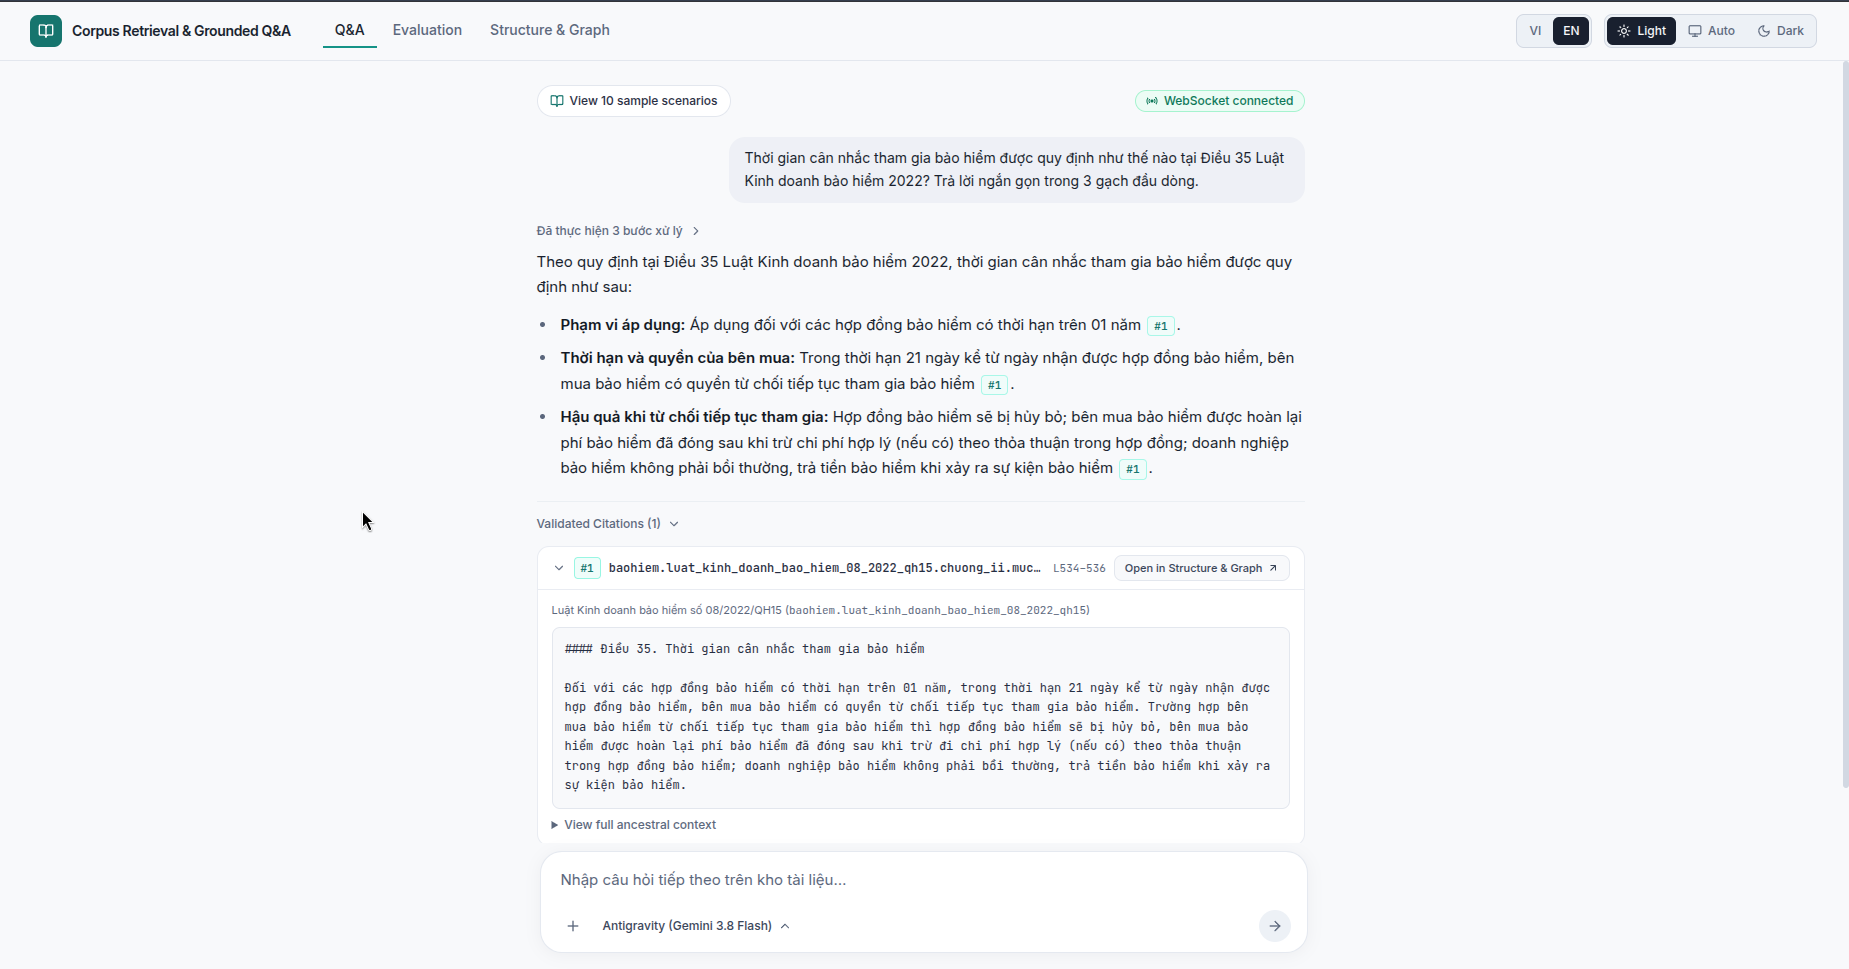
\includegraphics[width=\textwidth]{figures/ui_grounded_qa.png}
    \par\vspace{2pt}{\footnotesize (a) Không gian Hỏi đáp có kiểm chứng trích dẫn (\texttt{Grounded Q\&A}) và luồng sự kiện MCP}
\end{minipage}\hfill
\begin{minipage}[t]{0.485\textwidth}
    \centering
    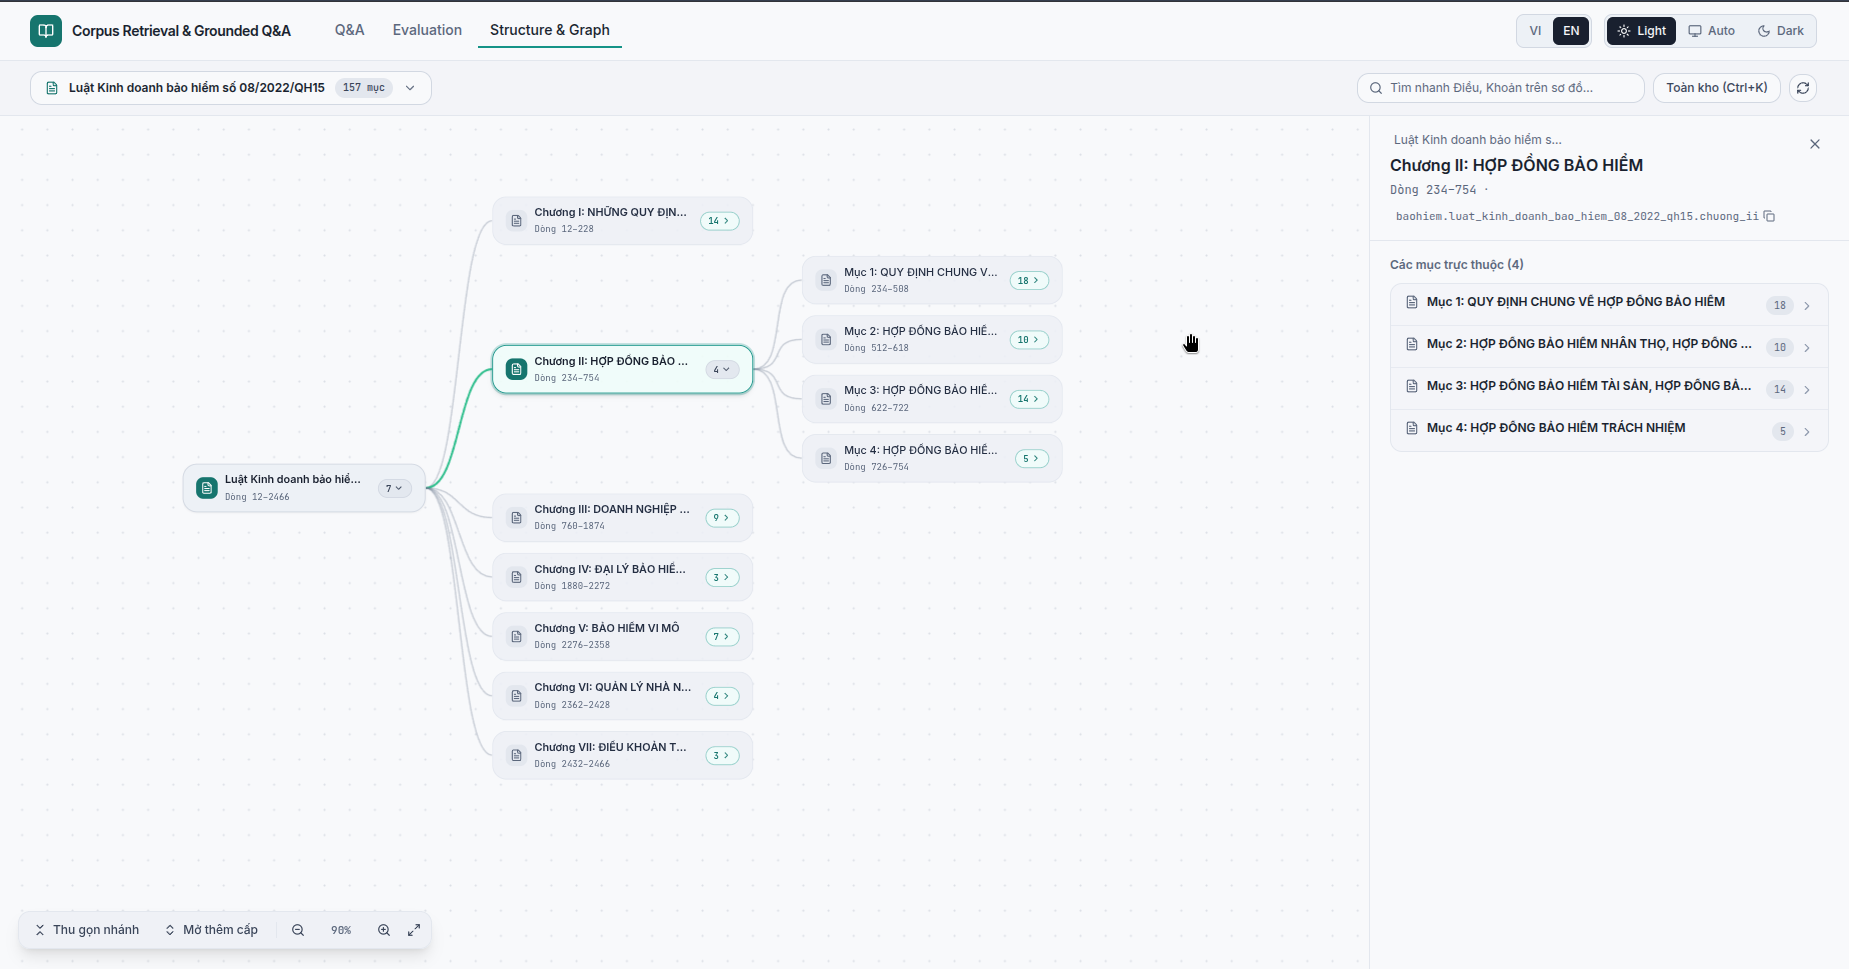
\includegraphics[width=\textwidth]{figures/ui_explorer_graph.png}
    \par\vspace{2pt}{\footnotesize (b) Không gian khám phá cây phân cấp \texttt{ltree}, đối chiếu dòng nguyên bản 1:1 và Knowledge Graph}
\end{minipage}
\caption{Giao diện thực tế của hệ thống Corpus \& Graph Observatory Dashboard (\texttt{uv run rag-eval ui})}
\label{fig:ui_dashboard}
\end{figure}

\begin{table}[H]
\centering
\caption{Mẫu 6 truy vấn kiểm thử tiêu biểu trong bộ đánh giá 100 câu}
\label{tab:sample_queries}
\scriptsize\setlength{\tabcolsep}{3.5pt}\begin{tabularx}{\textwidth}{ll>{\raggedright\arraybackslash}X>{\raggedright\arraybackslash}p{3.0cm}>{\raggedright\arraybackslash}p{3.9cm}c}
\toprule
\textbf{Mã} & \textbf{Bộ / Miền} & \textbf{Câu hỏi tóm tắt} & \textbf{\texttt{query} / \texttt{pattern}} & \textbf{Đường dẫn \texttt{ltree} đích} & \textbf{Giỏ / Hạng} \\
\midrule
\texttt{e001} & \texttt{TS1}\newline Next.js & Cờ \texttt{--yes} của \texttt{create-next-app} cấu hình mặc định import alias và bundler nào? & \texttt{create-next-app --yes...}\newline\texttt{pattern: "--yes"} & \nolinkurl{nextjs.01_getting_started.01_installation.quick_start} & \texttt{both}\newline (\#1) \\
\addlinespace[2pt]
\texttt{e021} & \texttt{TS1}\newline Next.js & Truyền \texttt{FormData} của Server Action vào \texttt{Object.fromEntries} sinh ra các thuộc tính nội bộ có tiền tố gì? & \texttt{Server Action FormData...}\newline\texttt{pattern: "\$ACTION"} & \nolinkurl{nextjs.02_guides.forms.how_it_works} & \texttt{verbatim}\newline (\#1) \\
\addlinespace[2pt]
\texttt{e029} & \texttt{TS1}\newline Node.js & Trên Windows, khi \texttt{options.env} của \texttt{spawn} chứa cả khóa \texttt{PATH} và \texttt{Path}, Node.js chọn khóa nào? & \texttt{child\_process spawn...}\newline\texttt{pattern: "options.env"} & \nolinkurl{nodejs.child_process.overview} & \texttt{both}\newline (\#1) \\
\addlinespace[2pt]
\texttt{e053} & \texttt{TS2}\newline Next.js & Vì sao triển khai nhiều replica Next.js tự host gây lỗi \texttt{Failed to find Server Action} và cần biến môi trường nào? & \texttt{self-hosting multiple...}\newline\texttt{pattern: "NEXT\_SERVER\_..."} & \nolinkurl{nextjs.02_guides.self_hosting.multi_server_deployments.server_functions_encryption_key} & \texttt{both}\newline (\#1) \\
\addlinespace[2pt]
\texttt{e072} & \texttt{TS2}\newline Next.js & Trong kiến trúc Multi-Zones, vì sao liên kết giữa các zone phải dùng thẻ \texttt{<a>} và tránh đụng độ tài nguyên tĩnh thế nào? & \texttt{Multi-Zones links...}\newline\texttt{pattern: "assetPrefix"} & \nolinkurl{nextjs.02_guides.multi_zones.linking_between_zones} & \texttt{semantic}\newline (\#2) \\
\addlinespace[2pt]
\texttt{e083} & \texttt{TS2}\newline Node.js & Sau khi monkey-patch CommonJS export của \texttt{node:fs}, làm sao đồng bộ lại các named exports bên ES module? & \texttt{syncBuiltinESM...}\newline\texttt{pattern: "syncBuiltin..."} & \nolinkurl{nodejs.module.the_module_object.module_syncbuiltinesmexports} & \texttt{verbatim}\newline (\#1) \\
\bottomrule
\end{tabularx}
\end{table}

\vspace{0.3cm}
\begin{center}
\begin{tabular}{p{0.45\textwidth}p{0.45\textwidth}}
\centering \textbf{GIẢNG VIÊN HƯỚNG DẪN} & \centering\arraybackslash \textbf{ĐẠI DIỆN NHÓM THỰC HIỆN} \\
\centering \textit{Ký và ghi rõ họ tên} & \centering\arraybackslash \textit{Ký và ghi rõ họ tên} \\[1.8cm]
\centering \textbf{ThS. Nguyễn Văn Sơn} & \centering\arraybackslash \textbf{Đinh Việt Hoàng}
\end{tabular}
\end{center}


\end{document}
